% % % % % % % %  MDT UFSM 2015  % % % % % % % % 
%% Arquivo base para o documento - ver. 1.08 %%
% % % % % % % % % % % % % % % % % % % % % % % % 


% % % OPCOES DE COMPILACAO
% % % PAGINACAO
% % % PAGINACAO SIMPLES (FRENTE): PARA TRABALHOS COM MENOS DE 100 PAGINAS
\documentclass[oneside,openright,12pt]{ufsm_2015} %%%%% OPCAO PADRAO -> PAGINACAO SIMPLES. PARA TRABALHOS COM MAIS DE 100 PAGINAS COMENTE ESTA LINHA E DESCOMENTE A LINHA 
% % % % % % % % % % % % % % % % % % % % % % % % % % % % % % % % % % % % % % %
% PAGINACAO DUPLA (FRENTE E VERSO): PARA TRABALHOS COM MAIS DE 100 PAGINAS
% \documentclass[twoside,openright,12pt]{ufsm_2015}  %%%% PARA TRABALHOS COM MAIS DE 100 PAGINAS DESCOMENTE AQUI
% % % % % % % % % % % % % % % % % % % % % % % % % % % % % % % % % % % % %




% % % %  CODIFICACAO DO TEXTO 
% % % %  POR PADRAO USA-SE UTF8. PARA APLICAR A CODIFICACAO OESTE EUROPEU (ISO 8859-1) DESCOMENTE A LINHA ABAIXO. ELA ATIVA A OPCAO "latin1" DO PACOTE "inputenc"
% \oesteeuropeu
% % % % % % % % % % % 



% % % % % % % % PACOTES PESSOAIS % % % % % % % %  

\usepackage{minted}

\usepackage{caption}
\usepackage{subcaption}

\newcommand{\kotlinminted}[1]{\inputminted[breaklines=true, baselinestretch = 0.9]{kotlin}{E:/Git/Easy-Tracker-Android-App/app/src/main/java/com/example/startracker/#1}}

\newcommand{\arduinominted}[1]{\inputminted[breaklines=true, baselinestretch = 0.9]{arduino}{E:/Git/Easy-Tracker-System/src/main/#1}}

\newcommand{\xmlminted}[1]{\inputminted[breaklines=true, baselinestretch = 0.9]{xml}{E:/Git/Easy-Tracker-Android-App/app/src/main/res/layout/activity_main.xml}}

%Please add the following packages if necessary:
\usepackage{booktabs, multirow} % for borders and merged ranges
\usepackage{makecell}
%\usepackage{changepage,threeparttable} % for wide tables



% % % % % % % % DEFINICOES PESSOAIS % % % % % % % %







% % % % % % % % % % % % % % % % % % % % % % % % % % % % % % % % % % % % % % % % % % % 











% % % % % % % % % % % % % % % % % % % % % % % % % % % % % % % % % 
% % % % % % % % % % % % DADOS DO TRABALHO % % % % % % % % % % % % 
% % % % % % % % % % % % % % % % % % % % % % % % % % % % % % % % % 

% % % % % % % % % % INFORMACOES INSTITUCIONAIS % % % % % % % % % % 


% % CENTRO DE ENSINO DA UFSM
\centroensino{Centro de Tecnologia}  %%% NOME POR EXTENSO
\centroensinosigla{CT}  %%% SIGLA

% % CURSO DA UFSM
\nivelensino{Graduação}  %%%%%%% NIVEL DE ENSINO 
\curso{Engenharia de Computação}   %%%%% NOME POR EXTENSO
\ppg{EC}   %%%%%% SIGLA
\statuscurso{Curso}  %%%% STATUS= {Programa} ou {Curso}
% \EAD  %%%% para cursos EAD
% % % %  LOCAL DO CAMPUS OU POLO
\cidade{Santa Maria}
\estado{RS}


% % % % % % % % % % INFORMACOES DO AUTOR % % % % % % % % % % 
\author{Eugênio Piveta Pozzobon}   %%%%% AUTOR DO TRABALHO
\sexo{M} %%%% SEXO DO AUTOR -> M=masculino   F=feminino (IMPORTANTE PARA AJUSTAR PAGINAS PRE-TEXTUAIS)
\grauensino{Graduação}    %%%%%%%% GRAU DE ENSINO A SER CONCLUIDO
\grauobtido{Bacharel}    %%%%% TITULO OBTIDO
\email{eugeniopp00@gmail.com}   %%%% E-MAIL PARA CATALOGRAFICA (COPYRIGHT) - OBRIGATORIO
%\endereco{Rua das abobrinhas, n. 666} %%%% TELEFONE PARA CATALOGRAFICA (COPYRIGHT) (CAMPO OPICIONAL -- CASO NAO POSSUA OU NAO QUEIRA DIVULGAR COMENTE A LINHA)
\fone{+55 55 99620-2527}   %%%% TELEFONE PARA CATALOGRAFICA (COPYRIGHT) FORMATO {11 2222 3333} (CAMPO OPICIONAL -- CASO NAO POSSUA OU NAO QUEIRA DIVULGAR COMENTE A LINHA)
%\fax{11 2222 3333}   %%%% FAX PARA CATALOGRAFICA (COPYRIGHT) FORMATO {11 2222 3333} (CAMPO OPICIONAL -- CASO NAO POSSUA OU NAO QUEIRA DIVULGAR COMENTE A LINHA)


% % % % % % % % % % INFORMACOES DA BANCA % % % % % % % % % % 
% OBSERVACOES: O CAMPO ORIENTADOR EH OBRIGATORIO E NAO DEVE SER COMENTADO
% % % % % %    OS DEMAIS MEMBROS DA BANCA (COOREIENTADOR E DEMAIS PROFESSORES) QUANDO COMENTADOS NAO APARECEM NA FOLHA DE APROVACAO (O LAYOUT DA FOLHA DE APROVACAO ESTA PREPARADO PARA O ORIENTADOR E ATE MAIS 4 MEMBROS NA BANCA
\orientador{Rafael Concatto Beltrame}{Dr}{UFSM}{M}{P}  %%%INFORMACOES SOBRE ORIENTADOR: OS CAMPOS SAO:{NOME}{SIGLA DA TITULACAO}{SIGLA DA INSTITUICAO DE ORIGEM}{SEXO} M=masculino   F=feminino {PARTE DA BANCA?} P=presidente  M=Membro  N=Nao faz parte

% \coorientador{Maria da Costa}{Dra}{AAAA}{F}{M} %%%INFORMACOES SOBRE CO-ORIENTADOR: OS CAMPOS SAO:{NOME}{SIGLA DA TITULACAO}{SIGLA DA INSTITUICAO DE ORIGEM}{SEXO} M=masculino   F=feminino {PARTE DA BANCA?} P=presidente  M=Membro  N=Nao faz parte

% \bancaum{Banca Um}{Dr}{AAAA}{F}{M}  %%%INFORMACOES SOBRE PRIMEIRO NOME DA BANCA: OS CAMPOS SAO:{NOME}{SIGLA DA TITULACAO}{SIGLA DA INSTITUICAO DE ORIGEM}{SEXO} M=masculino   F=feminino {PARTE DA BANCA?} P=presidente  M=Membro  N=Nao faz parte

% \bancadois{Banca Dois}{Dr}{BBBB}  %%%INFORMACOES SOBRE SEGUNDO NOME DA BANCA: OS CAMPOS SAO:{NOME}{SIGLA DA TITULACAO}{SIGLA DA INSTITUICAO DE ORIGEM}
% \bancatres{Banca Três}{Dra}{CCCC} %%%INFORMACOES SOBRE TERCEIRO NOME DA BANCA: OS CAMPOS SAO:{NOME}{SIGLA DA TITULACAO}{SIGLA DA INSTITUICAO DE ORIGEM}
% \bancaquatro{Banca Quatro}{Dr}{DDDD} %%%INFORMACOES SOBRE QUARTO NOME DA BANCA: OS CAMPOS SAO:{NOME}{SIGLA DA TITULACAO}{SIGLA DA INSTITUICAO DE ORIGEM}
% \bancacinco{Banca Cinco}{Dra}{EEEE} %%%INFORMACOES SOBRE QUARTO NOME DA BANCA: OS CAMPOS SAO:{NOME}{SIGLA DA TITULACAO}{SIGLA DA INSTITUICAO DE ORIGEM}
% \supervisor{Al Paccino}{Dr}{MAFIA}{M}{N} %%%INFORMACOES SOBRE SUPERVISOR (indicado para estagios): OS CAMPOS SAO:{NOME}{SIGLA DA TITULACAO}{SIGLA DA INSTITUICAO DE ORIGEM}{SEXO} M=masculino   F=feminino {PARTE DA BANCA?} P=Presidente  M=Membro  N=Nao faz parte



% % % % % % % % % % REALIZACAO POR VIDEO CONFERENCIA (MEMORANDO 04/2016 BIBLIOTECA CENTRAL UFSM)
% \videoconferencia % % % % QUANDO O ACADEMICO DEFENDE POR VIDEO CONFERENCIA (PERMITIDO PELO ARTIGO 82 DO REGIMENTO GERAL DA PRPGP/UFSM). PARA DEFESAS NAS QUAIS O ACADEMICO ESTA PRESENTE COMENTE ESTA LINHA
% % % % QUANDO UM DOS MEMBROS DA BANCA PARTICIPA POR VIDEO CONFERENCIA INDICAR O MEMBRO DE ACORDO COM A LISTA ABAIXO. CASO CONTRARIO MANTER A PALAVRA "NAO". SAO PERMITIDOS, PELO REGIMENTO PRGPGP (ARTIGO 83) ATE 2 MEMBROS 
\videoconferenciabancap{NAO}  %%%% PRIMEIRO MEMBRO
\videoconferenciabancas{NAO}  %%%%% SEGUNDO MEMBRO
% % O > ORIENTADOR
% % CO > COORIENTADOR% % % % QUANDO UM DOS MEMBROS DA BANCA PARTICIPA POR VIDEO CONFERENCIA INDICAR O MEMBRO DE ACORDO COM A LISTA ABAIXO. CASO CONTRARIO MANTER A PALAVRA "NAO". SAO PERMITIDOS, PELO REGIMENTO PRGPGP ATE 2 MEMBROS.
% % 1 > BANCA UM
% % 2 > BANCA DOIS
% % 3 > BANCA TRÊS
% % 4 > BANCA QUATRO
% % 5 > BANCA CINCO
% % S > SUPERVISOR
% % % % % % % % % % % % % % % % % % % % % % % % % % % % % % % % % % % % 



% % % % % % % % % % INFORMACOES SOBRE O TRABALHO % % % % % % % % % %
% % % %  TITULO DO TRABALHO
\titulo{Desenvolvimento de uma Plataforma Equatorial de Baixo Custo para Astrofotografia} %% NAO EH NECESSARIO CAPITALIZAR
% % % %  TITULO DO TRABALHO EM INGLES
\englishtitle{Desenvolvimento de uma Plataforma Equatorial de Baixo Custo para Astrofotografia}  %% NAO EH NECESSARIO CAPITALIZAR
% % % AREA DE CONCENTRACAO DO TRABALHO (CNPQ)
\areaconcentracao{Engenharia de Computação}
% % % TIPO DE TRABALHO - MANTER APENAS UMA LINHA DESCOMENTADA
%\tccg  %% Tese de <nivel de ensino>
% \qualificacao %% Exame de Qualificação de <nivel de ensino>
% \dissertacao %% Dissertacao de <nivel de ensino>
% \monografia %% Monografia
% \monografiag  %% Monografia (nao exibe area de concentracao)
% \tf  %% Trabalho Final de <nivel de ensino>
% \tfg  %% Trabalho Final de Graduacao (nao exibe area de concentracao)
% \tcc  %% Trabalho de Conclusao de Curso
% \tccg  %% Trabalho de Conclusao de Curso (nao exibe area de concentracao)
% \relatorio  %% Relatório de Estágio (nao exibe area de concentracao)
\generico   %%% Alternativa para aqueles cursos que nao recebem o titulo de bacharel ou licenciado. Ex: engenharia, arquitetura, etc... Os campos abaixo tambem devem ser preenchidos
     \tipogenerico{Trabalho de Conclusão de Curso}
     \tipogenericoen{Tipo de trabalho em inglês}
     \concordagenerico{o}
     \graugenerico{Engenheiro de Computação}
% % % DATA DA DEFESA 
\data{00}{00}{2022} %% FORMATO {DD}{MM}{AAAA}



% % % % %  ALGUMAS ENTRADAS PRE-TEXTUAIS
% % % % CASO NAO QUEIRA UTILIZA-LAS COMENTE A LINHA DE COMANDO
% % % EPIGRAFE
%\epigrafe{"Se você tem uma maçã e eu tenho uma maçã e formos trocar essas maçãs, você e eu ainda teremos uma maçã cada um. Mas se você tem uma ideia e eu tenho uma ideia e formos trocar essas ideias, cada um de nós terá duas ideias."}{George Bernard Shaw} %ESTRUTURA DE CAMPOS -> {Texto}{Autor}
% % % DEDICATORIA
%\dedicatoria{Dedico este trabalho a todos os astrofotógrafos que carecem de recursos para investir em equipamentos, na esperança de que isso possa ajudá-los a produzir fotografias de qualidade, alcançando ainda mais longe no céu profundo.}
% % % %  AGRADECIMENTOS
% \agradecimentos{A mim!}

% % % % %  RESUMO E PALAVRAS CHAVE DO RESUMO - OBRIGATORIO PARA MDT-UFSM
\resumo{
% \singlespacing
Atualmente, a astrofotografia é realizada por telescópios monumentais e também por um grande número de astrofotógrafos amadores, e estes contam com inúmeros desafios. O principal deles reside no fato que corpos celestes, de forma geral, demandam elevados tempos de exposição. Infelizmente, caso a câmera esteja imóvel sobre um tripé, o movimento de rotação da Terra não permite que os astros sejam expostos ao sensor por muito tempo, pois as imagens acabam borradas. Por esse motivo, é necessário o uso de uma ferramenta que movimente a câmera no sentido de rotação aparente do céu, compensando esse movimento e obtendo-se um registro fotográfico de alta qualidade. Para isso, existem inúmeras ferramentas comerciais para o rastreamento do céu, porém, todas elas são comercializadas no hemisfério Norte e com um custo excessivo para o brasileiro médio. Então, a fim de simplificar e reduzir o custo associado à astrofotografia, tornando-a acessível, objetivou-se com este trabalho desenvolver uma plataforma equatorial para astrofotografia que seja portátil; robusta; precisa; de fácil configuração e utilização; de peso e volume compatíveis com tripés fotográficos; e com custo inferior à soluções comerciais. A plataforma tem como diferencial um aplicativo mobile que descomplica o uso dessas ferramentas para configuração e setup da plataforma para a obtenção de registros fotográficos. O sistema final passou por testes de vibração para garantir que a montagem estaria adequada para o uso, e também com testes em campo, onde foram tiradas fotografias da via-láctea, comparando-se resultados fotográficos com e sem o uso da plataforma desenvolvida.


}
\palavrachave{Astrofotografia. Plataforma Equatorial. Sistema Eletrônico. Aplicativo Android. Bluetooth.}
% "... deverão constar, no mínimo, três palavras-chave, iniciadas em
% letras maiúsculas, cada termo separado dos demais por ponto, e
% finalizadas também por ponto." MDT 2012

% % % % %  ABSTRACT E PALAVRAS CHAVE DO RESUMO - OBRIGATORIO PARA MDT-UFSM
\abstract{
Currently, astrophotography remains practiced by large telescopes and also by astrophotographers that have countless challenges. The main one relies on the fact that celestial bodies, in general, demand long exposure times. Unfortunately, despite the camera being on a tripod, the rotational movement of the Earth doesn't allow the stars to be exposed to the sensor for a long time, resulting in blurry images. For this reason, it is necessary to use a tool that moves the camera in the apparent rotation direction of the sky, compensating for this movement and obtaining a high-quality photographic record. For this, there are numerous commercial tools for tracking the sky. However, all of them are commercialized in the Northern hemisphere and with an exorbitant cost for the average Brazilian. So, in order to simplify and reduce the cost associated with astrophotography, making it accessible, the objective of this work was to develop an equatorial platform for astrophotography that is portable; robust; precise; easy to set up and use; of weight and volume compatible with photographic tripods; and at a lower cost than commercial solutions. The platform's differential is a mobile application that makes it easy to use these tools for the configuration of the platform to obtain photographic records. The final system has been passed into vibration tests to ensure that the assembly would be suitable for use.  Also, the system got tested with long exposure photography.
}
\keywords{Astrophotography. Equatorial Mount. Electronic System. Android Application. Bluetooth.}


% % %  ATIVACAO DE LISTAS E PAGINAS ESPECIAIS
% % %  PARA QUE APARECAO NAO NO TEXTO DESCOMENTE A LINHA ABAIXO -> POR PADRAO TODAS ESTAO ATIVIDADAS

% % LISTA DE FIGURAS 
% \semfiguras   %%(QUANDO ATIVIDA NAO EXIBE A LISTA)
% % LISTA DE GRAFICOS 
 \semgraficos   %%(QUANDO ATIVIDA NAO EXIBE A LISTA)
% % LISTA DE ILUSTRACOES 
 \semilustracoes  %%(QUANDO ATIVIDA NAO EXIBE A LISTA)
% % LISTA DE TABELAS 
% \semtabelas   %%(QUANDO ATIVIDA NAO EXIBE A LISTA)
% % LISTA DE QUADROS 
 \semquadros   %%(QUANDO ATIVIDA NAO EXIBE A LISTA)
% % LISTA DE APENDICES 
% \semapendices  %%(QUANDO ATIVIDA NAO EXIBE A LISTA)
% LISTA DE ANEXOS 
% \semanexos   %%(QUANDO ATIVIDA NAO EXIBE A LISTA)



% % % %  LISTA DE ABREVIATURAS E SIGLAS
%%%%%%%% OBS: O espaco entre colchetes \item[] e um ambiente matematico
%%%%%%%% para não utilizar comente as linhas abaixo.
%\siglamax{SIGLAMAX} %%%% coloque aqui a maior sigla %(indentacao)
%\listadeabreviaturasesiglas{
%\item[SIGLA1]	Nome Completo da Sigla 1
%\item[SIGLA2]	Nome Completo da Sigla 2
%\item[SIGLAMAX]	Nome Completo da Sigla MAX
%}

% % % %  LISTA DE SIMBOLOS
%%%%%%%% OBS: O espaco entre colchetes \item[] e um ambiente matematico
%%%%%%%% para não utilizar comente as linhas abaixo.
%\simbolomax{(Re)2} %%%% coloque aqui o maior simbolo (indentacao)
%\listadesimbolos{
%\item[u_*]	Escala de velocidade de fricção	
%\item[w_*]	Escala de velocidade convectiva
%\item[(Re)^2]	Maior simbolo da lista
%}


% % % FICHA CATALOGRAFICA
\semcatalografica  %%%%  (QUANDO ATIVIDA NAO EXIBE A FICHA CATALOGRAFICA NECESSITA DO ARQUIVO DA FICHA: ficha_catalografica.pdf
% % % A FICHA CATALOGRAFICA FORNECIDA PELA UFSM EH UM PDF DO TAMANHO A4
% % % EH POSSIVEL GERA-LA NO SITE http://cascavel.ufsm.br/ficha_catalografica/
% % % OS COMANDOS ABAIXO DEFINEM AS MARGENS PARA CORTAR A FICHA FORNECIDA E COLOCA-LA COMO UMA FIGURA NO DOCUMENTO LATEX
\margemesquerda{4}   %%%% CORTE DE MARGEM ESQUERDA EM CM
\margemdireita{1.5}   %%%% CORTE DE MARGEM DIREITA EM CM
\margemsuperior{17}  %%%% CORTE DE MARGEM SUPERIOR EM CM
\margeminferior{3} %%%% CORTE DE MARGEM INFERIOR EM CM
% % %  DICA: IMPRIMA UMA COPIA DA FICHA CATALOGRAFICA E FACA A MEDIDA DAS MARGENS!





% % FOLHA DE ERRADA (versao rudimentar...pode ser aprimorado)
% % para não utilizar comente as linhas abaixo.
% % deve ser preenchida como um ambiente tabular de quatro colunas:
% % pagina & linha & onde se le & leia-a se \\

%\errata{
%10   &    10    & errado   & certo \\
%\hline
%12    &    5     & errado com um texto mais longo & certo %agora com um texto mais longo\\
%\hline
%13   &    3    & $x^2$   & $2x$\\
%}

% % % % % % % % % % % % % % % % % % % % % % % % % % % % % % % % % % % % % % % % % % % % % % 


% % % % % % % % % % % % % % % % % % % % % % % % % % % % % % % % % % % % % % 
% % % % % % % % % % % %  OPCOES DE FORMATACAO % % % % % % % % % % % % % % %
% % % % % % % % % % % % % % % % % % % % % % % % % % % % % % % % % % % % % % 
% % % CAPITULO: por padrao alinhado a esquerda. Para ativar alinhamento centralizado descomente o comando abaixo

% \centralizado  %%%% <<< centraliza todos os capitulos

% % % % % % % % % % % % % % % % % % % % % % % % % % % % % % % % % % % % % %
% % % FONTES: descomente uma das opcoes. caso nenhuma seja ativada a clase usara a fonte padrao do latex

%% helvetica
\usepackage[scaled]{helvet}
\renewcommand*\familydefault{\sfdefault}

%% arial
% \renewcommand{\rmdefault}{phv} % Arial
% \renewcommand{\sfdefault}{phv} % Arial

%%times
\usepackage{mathptmx}

% % % % % % % % % % % % % % % % % % % % % % % % % % % % % % % % % % % % % % 
% % % % % % % % % % % % % % % % % % % % % % % % % % % % % % % % % % % % % % 
% % % % % % % % % % % % % % % % % % % % % % % % % % % % % % % % % % % % % % 
% % % % % % % % % % % % % % % % % % % % % % % % % % % % % % % % % % % % % % 


% % % % % % % % % % % % % % % % % % % % % % % % % % % % % % % % % % % % % % 
% % % % % % % % % % % % % % % % % % % % % % % % % % % % % % % % % % % % % % 
% % % % % % % % % % % %  INICIO DO DOCUMENTO  % % % % % % % % % % % % % % %
% % % % % % % % % % % % % % % % % % % % % % % % % % % % % % % % % % % % % % 
% % % % % % % % % % % % % % % % % % % % % % % % % % % % % % % % % % % % % %


\begin{document}



% % % % % % % % % % % % % % % % % % % % % % % % % % % % % % % % % % % % % % 
\pretextual  %%%% GERA AS PAGINAS PRE-TEXTUAIS   
% % % % % % % % % % % % % % % % % % % % % % % % % % % % % % % % % % % % % % 

% % % % % % % % % % % % % % % % % % % % % % % % % % % % % % % % % % % % % % 
% % % % % CORPO DO TRABALHO - INCLUA OS SEUS TEXTOS AQUI
% % % % % SUGESTAO -> UTILIZE ARQUIVOS EXTERNOS A PARTIR DO COMANDO \input
% % % % % % % % % % % % % % % % % % % % % % % % % % % % % % % % % % % % % % 
% % % % % % % % % % INICIO DAS PAGINAS TEXTUAIS % % % % % % % % % % % % % % 
% % % % % % % % % % % % % % % % % % % % % % % % % % % % % % % % % % % % % % 

\chapter{Introduçao}

Desde os primeiros registros datados, civilizações já observavam o céu e, desse modo, podiam contabilizar a passagem do tempo, identificar as estações do ano, os ciclos sazonais de chuvas e/ou secas, etc. Assim, por exemplo, era possível realizar um planejamento mais assertivo acerca da melhor época de plantio e colheita de diferentes culturas. Cada civilização tinha seu meio e técnica de observação. Por exemplo, em 4000 a.C., os povos da Mesopotâmia utilizavam zigurates para observar o céu noturno ; já em 2500 a.C., foi construída a estrutura de pedras Stonehenge, na Inglaterra, para registrar os solstícios. Foi somente em 1609 d.C. que Galileu conseguiu aperfeiçoar e utilizar um telescópio refrator para observar os planetas e as estrelas pela primeira vez. \cite{site:brescolaAstrofoto}

A astrofotografia consiste no emprego de técnicas fotográficas para registrar objetos astronômicos, como planetas, estrelas, galáxias, nebulosas, etc. A primeira é datada de 1840 e é um registro da Lua. \cite{site:introCabau} Desse período em diante, a fotografia teve um papel muito importante na observação celeste e no registro do céu para análise científica. Essa técnica foi evoluindo gradualmente de forma que, por volta de 1960, já havia equipamentos que permitiam realizar registros mais concretos e eficientes, possibilitando fotos com mais definição e nitidez. \cite{site:importanciaAstroftoSantos}

No fim do século XX, telescópios maiores e mais complexos, instalados na Terra ou a orbitando no espaço (como o telescópio espacial Hubble), ampliaram a capacidade da ciência em estudar fenômenos astronômicos ou mesmo a origem do próprio universo. \cite{site:importanciaAstroftoSantos}
Paralelamente, as ferramentas amadoras para astronomia (como telescópios de baixo custo), ou mesmo para astrofotografia (câmeras de custo mais acessível e equipamentos para rastreamento do céu) continuaram a ser desenvolvidas, de forma que um grande número de astrônomos e, especificamente, astrofotógrafos amadores continuassem exercendo seu hobby ou mesmo contribuindo à ciência.

Nesse sentido, o desenvolvimento de equipamentos acessíveis voltados ao público amador tem um papel fundamental para despertar o interesse pela ciência em cada vez mais pessoas. Atualmente, o custo de muitas ferramentas classificadas como “amadoras” ainda é elevado, principalmente para a realidade brasileira. Como exemplo, hoje podem ser empregados pequenos telescópios comerciais ou artesanais acoplados a câmeras digitais (de celular ou DSLRs (Digital Single Lens Reflex). No entanto, os principais desafios de se fotografar galáxias, nebulosas, etc., é que esses corpos, de forma geral, demandam elevados tempos de exposição.\cite{site:introCabau} Infelizmente, o movimento de rotação da Terra não permite que os astros sejam expostos ao sensor por muito tempo, pois as imagens ficariam borradas. Por esse motivo, é necessário o uso de uma ferramenta que movimente a câmera (acoplada ou não a um telescópio) no sentido de rotação aparente do céu, compensando o movimento e permitindo que o sensor da câmera possa receber luz por longos períodos de tempo (de minutos a horas).\cite{site:introCabau} Assim, consegue-se obter um registro fotográfico de alta qualidade e com um baixo custo computacional de pós processamento.


Nesse sentido, existem inúmeras ferramentas comerciais para o rastramento rastreamento do céu voltadas ao público amadador, como Nyx Track, SkyGuiderTM Pro, PolarieTM, entre outras (conforme Figura \ref{fig:skyguider}). Porém, todas elas são comercializadas no hemisfério norte e com um custo excessivo para brasileiro médio (considerando taxa de câmbio, taxas de importação e frete). Assim, de modo a contribuir à popularização da astrofotografia no Brasil, incentivando cada vez mais jovens a seguirem na carreira científica, propõe-se o desenvolvimento de uma plataforma equatorial de baixo custo para astrofotografia.


\begin{figure}[htb]
	\centering
	\caption{Exemplo de solução comercial empregada em astrofotografias. }
	\includegraphics[width=0.3\linewidth]{figuras/skyguider}
	\label{fig:skyguider}
	\fonte{\cite{site:ioptron}}
\end{figure}


\chapter{Desenvolvimento Teórico}

\section{Astrofotografia}

A astrofotografia é um ramo da astronomia e da fotografia que combina toda a ciência envolvida na documentação e registro de estrelas, constelações, planetas, meteoros, etc., com a arte da fotografia. Dentro da astrofotografia, existem variantes como planetária, solar e céu profundo \cite{livro:astropratica}. Além disso, existem diferenças entre a astrofotografia praticada profissionalmente por cientistas, em grandes telescópios, da praticada por amadores. Porém, ambas as atividades são importantes e se complementam.

As fotografias capturadas por telescópios profissionais possuem vantagens no fato como uma grande ampliação, além de foco e definição, devido aos grandes espelhos que compõe suas montagens. Contudo, isso se torna um problema para a captura de imagens mais amplas. Essas fotografias são registradas, em sua maioria, por astrofotógrafos amadores \cite{livro:astropratica}.

Além disso, a astrofotografia amadora também precisa de equipamentos que, no Brasil, custam um preço que acaba afastando uma boa parcela da população dessa prática.

\subsection{Equipamentos}

Além de uma câmera e uma lente, existem alguns equipamentos periféricos que são fundamentais para a prática da astrofotografia: tripé e disparador remoto (intervalômetro) para a câmera. O tripé é responsável por manter a câmera estável durante o registro das estrelas; o Disparador tem a função de operar a câmera remotamente para evitar que haja o operador faça a câmera tremer ao apertar algum botão e/ou também permitir a utilização do modo \textit{Bulb} das DSLR. O modo \textit{Bulb} consiste em permitir um controle total do tempo de exposição pelo operador \cite{book:bbcsky}.

\subsubsection{Câmeras}

As câmeras digitais possuem sensores CMOS (\textit{Complementary Metal-Oxide Semi-conductor}) de imagem que substituem o filme das máquinas fotográficas mais antigas. O sensor CMOS pode ter diversos tamanhos físicos diferentes e uma densidade de \textit{pixels} por polegada (dpi) diversa entre os modelos. Por norma, quanto maior for o sensor físico, mais qualidade terá a imagem final \cite{man:vanessacameras}.

Existem diversos modelos de câmeras para fotografia: compacta, super-zoom, \textit{mirrorless}, DLSR e por fim as câmeras em celulares. As câmeras \textit{mirrorless} atualmente são equiparáveis às DSLR e ambas são as mais usadas para astrofotografia, possibilitam trocar lentes e podem ser utilizadas para capturar de céu noturno. Além disso, possibilitam uma série de configurações em modo manual que não são possíveis em câmeras semi-profissionais, compactas ou de super-zoom \cite{book:bbcsky}.

\subsubsection{Lentes}
A lente é um equipamento acoplado no corpo da câmera que é responsável por focalizar a luz que invade o sensor. As lentes podem ser rígidas no corpo da câmera, no caso de modelos semi-profissionais e compactos; ou podem ser removíveis para o caso de modelos profissionais. Nesse último caso, as lentes removíveis são itens que podem ser obtidos por escolha do fotógrafo e existe uma variedade de modelos.

Esses modelos podem ser lentes fixas ou \textit{zoom}. O primeiro é um modelo de lente que possui uma distância focal fixa. Já as lentes \textit{zoom} permitem uma variação na distância focal, o que acaba gerando o \textit{zoom} óptico \cite{man:claudia7licoes}. 

\paragraph{Distância Focal}

A distância focal de uma lente é um fator medido em milímetros e é o  que determina seu ângulo de visão. Quanto maior ele for, mais fechado será o ângulo, gerando um zoom. Do contrário, quanto menor for a distância focal, maior será o ângulo de visão e consequentemente menor será o zoom da lente. A figura \ref{fig:focaldistance} ilustra essa relação da distância focal \cite{man:claudia7licoes}.

\begin{figure}[htb]
	\centering
	\caption{Efeito de zoom gerado pela variação da distância focal}
	\includegraphics[width=0.7\linewidth]{figuras/claudia-distanciafocal}
	\label{fig:focaldistance}
	\fonte{\cite{man:claudia7licoes}}
\end{figure}

Em um contexto de astrofotografia, lentes mais abertas são úteis para capturar a Via-Láctea (Figura \ref{fig:vialactea4mmSony}). Para fotografias de constelações, nebulosas e planetas distantes da Terra, é necessário uma lente mais fechada, que possibilite o enquadramento com o zoom necessário, conforme o tamanho do astro a ser fotografado. (Figura \ref{fig:jupiterSony})

\begin{figure}[!htb]
	\centering
	\caption{Fotografia da Via Láctea com lente \textit{zoom} em configuração de 4mm.}
	\includegraphics[width=0.7\linewidth]{figuras/vialactea4mm}
	\label{fig:vialactea4mmSony}
	\fonte{Autor}
\end{figure}

\begin{figure}[!htb]
	\centering
	\caption{Fotografia de Júpiter e as Luas de Galileu com lente \textit{zoom} em configuração de 205mm.}
	\includegraphics[width=0.2\linewidth]{figuras/jupiter205mm_Luas}
	\label{fig:jupiterSony}
	\fonte{Autor}
\end{figure}

\subsection{Exposição}

A exposição de uma imagem se refere à quantidade de luz captada pelo sensor da câmera. Uma imagem muito clara é considerada superexposta, um caso onde o sensor recebeu muita luz. Ao contrário, uma imagem subexposta é uma fotografia escura que recebeu pouca luz. Existem 3 parâmetros configuráveis em uma câmera profissional que são determinantes para a exposição e também para a qualidade da foto final \cite{site:eduardoemonica}. De forma geral, conseguir a exposição ideal é o principal desafio da astrofotografia de céu profundo \cite{livro:astropratica}.


\subsubsection{Tempo de Exposição}

Para captar uma imagem, a câmera possui um dispositivo que permite a passagem de luz em direção ao sensor interno que capta a imagem. Uma fotografia de longa exposição significa que a câmera permaneceu captando luz por um longo intervalo de tempo \cite{book:bbcsky}. Porém, não é possível abusar de longas exposições em alguns casos, pois a imagem pode sair "borrada" (Figura \ref{fig:velocidade}). uma pessoa correndo precisa ser fotografada em uma fração de segundo e uma paisagem, ao contrário, pode ser capturada durante mais de um segundo se a câmera estiver imóvel em um tripé.  

\begin{figure}[!htb]
	\centering
	\caption{Impacto do tempo de exposição de captura para objetos em movimento}
	\includegraphics[width=0.7\linewidth]{figuras/velocidade}
	\label{fig:velocidade}
	\fonte{Adaptado de \cite{site:eduardoemonica}}
\end{figure}

\subsubsection{Abertura}

Esse é o diâmetro do diafragme da lente, que permite a passagem de luz para o sensor (Figura \ref{fig:abertura}). Isso determina um valor "f/número". Um baixo "f/número" como f/1.8, indica um alto valor de abertura e significa dizer que a câmera irá receber mais luz \cite{book:bbcsky}. A abertura também impacta na profundidade de campo (Figura \ref{fig:profundidade}), o que significa que um valor baixo também apresenta o ônus da dificuldade focalizar.

% TODO checar questão do alto numero ou baixo número

\begin{figure}[!htb]
	\centering
	\caption{Variações de abertura de uma lente}
	\includegraphics[width=0.7\linewidth]{figuras/abertura}
	\label{fig:abertura}
	\fonte{Adaptado de \cite{site:eduardoemonica}}
\end{figure}

\begin{figure}[h]
	\centering
	\caption{Impacto da abertura na profundidade de campo}
	\includegraphics[width=0.7\linewidth]{figuras/profundidade}
	\label{fig:profundidade}
	\fonte{Adaptado de \cite{site:eduardoemonica}}
\end{figure}

\subsubsection{Sensibilidade (ISO)}

O ISO é um padrão internacional para a sensibilidade do sensor das câmeras. Essa sensibilidade também é configurável no sistema da câmera no momento da fotografia. Um valor baixo de ISO significa que o sensor precisa de mais tempo de exposição para captar mais luz, ao mesmo tempo, que reduz o ruído na imagem. (Figura \ref{fig:iso})
Um valor de ISO alto implica que a imagem final terá muito ruído, mas possibilita que ela seja registrada com um baixo tempo de exposição \cite{book:bbcsky}. O ruído agregado pelo ISO também acaba prejudicando a fotografia, reduzindo o contraste e a saturação das imagens, o que também pode levar a posterização, que é o comprometimento total da fotografia, pois a foto perde resolução e criam-se falhas nos \textit{pixels} da imagem.


\begin{figure}[!htb]
	\centering
	\caption{Variações do ISO e o ruído agregado}
	\includegraphics[width=0.7\linewidth]{figuras/ISO}
	\label{fig:iso}
	\fonte{Adaptado de \cite{site:eduardoemonica}}
\end{figure}

\subsection{Formatos de Arquivos}

As câmeras profissionais possibilitam salvar as imagens em diferentes formatos de arquivos, que inclui formato RAW, JPG ou ambos. Os arquivos JPG são uma versão reduzida dos formatos RAW, onde se aplica um algoritmo de compressão de imagens que acaba gerando perca de informações. Desse modo, arquivos RAW possuem a informação completa do sensor, sem nenhum tipo de compactação e acabam sendo muito grandes, mas permitem uma pós-produção mais precisa que acaba resultando em uma imagem com mais qualidade e detalhes \cite{book:bbcsky}.

\subsection{Rastro de Estrelas}

O movimento de rotação da terra gera um movimento aparente no céu. Ao realizar uma fotografia de longa exposição, esse movimento será visível criando o efeito de rastro de estrelas ou \textit{star trail}. (Figura \ref{fig:startrail_example})

\begin{figure}[!htb]
	\centering
	\caption{Fotografia com a captura de um \textit{star trail}}
	\includegraphics[width=0.7\linewidth]{figuras/startrail_example}
	\label{fig:startrail_example}
	\fonte{Autor}
\end{figure}

\subsubsection{Tempo de Exposição Máximo}
\label{sec:TempoMax}

Existe um limite de tempo máximo para que uma câmera fixa permaneça capturando luz sem que ocorra o fenômeno de \textit{star trail}. Esse tempo máximo depende de vários fatores, mas os dois principais são a distância focal da lente e a posição da estrela.

A distância focal é importante pois uma lente com um longo comprimento amplia a imagem, da mesma forma que amplia o rastro das estrelas. Do contrário, lentes com ângulo mais aberto, de menor comprimento focal, fazem tudo parecer pequeno, incluindo o movimento das estrelas, e isso permite um tempo de exposição maior \cite{book:astrophotographyAmateur}.

A distância de um astro até a linha do equador celestial é chamada de declinação estrelar, sendo medida em graus. Quanto menor for essa distância, mais rápido a estrela aparenta se movimentar no céu. Seja a declinação simbolizada por $\sigma$, e a distância focal nomeado $F$, em milímetros , uma equação capaz de aproximar o limite do tempo de exposição é dada em (\ref{eq:timeexp}) \cite{book:astrophotographyAmateur}. Existem ainda outras metodologias que buscam aproximar o tempo máximo de exposição. 

\begin{equation}
	t_{max} = \dfrac{343}{F\cos(\sigma)}~~[s]
	\label{eq:timeexp}
\end{equation}



\paragraph{Regra dos 500}

A regra dos 500 é uma fórmula que se baseia apenas distância focal, e o cálculo do tempo máximo é dado pela equação \ref{eq:timeexp500}. É uma regra muito simples, mas que permite uma aproximação razoável sobre o tempo máximo de exposição. Existem variantes dessa regra que alteram a constante no numerador, como a regra dos 300 ou a regra dos 400 \cite{site:500xNPF}.

\begin{equation}
	t_{max} = \dfrac{500}{F}~~[s]
	\label{eq:timeexp500}
\end{equation}

\paragraph{Regra NPF}

A regra NPF é uma evolução da equação (\ref{eq:timeexp}), que considera múltiplos fatores para recalcular a constante do numerador
\cite{site:500xNPF}. O tempo de exposição máximo é calculado pela equação \ref{eq:npf} com base na abertura da lente ($ N $), na distância focal ($ F $), no tamanho em micrômetros do sensor da câmera ($ p $), na declinação da estrela para onde a câmera será apontada ($\sigma$), e um fator de multiplicação ($ k $). O fator $ k $ é mantido em 1, porém pode ser aumentado até 3 para obter imagens mais nítidas e contrastantes \cite{site:500xNPF}. 

\begin{equation}
	t_{max} = k \cdot \dfrac{16,9 N  + 0,1 F + 13,7 p}{F\cos(\sigma)}~~[s]
	\label{eq:npf}
\end{equation}

\subsection{Empilhamento de Fotos}

O fenômeno de \textit{star trail} gera a necessidade do uso de ferramentas para compensar o movimento da Terra e permitir uma fotografia de longa exposição sem que se crie rastro. Essa compensação pode ser feita por \textit{software}, realizando-se o empilhamento de fotos de curta exposição \cite{livro:astropratica}.

O empilhamento consiste na junção de múltiplas imagens capturadas com a câmera montada em um tripé ou em uma montagem motorizada, que possibilita o somatório da luz capturada com essas fotos. Esse método de processamento é relevante para qualquer astrofotografia e possibilita a redução de ruído usando imagens de calibração \cite{book:bbcsky}. Existem inúmeros programas capazes de realizar esse processo como \textit{Deep Sky Stacker}, \textit{Sequator}, entre outros.

A combinação das imagens no pós-processamento não gera uma imagem mais luminosa ou colorida, o objetivo da combinação é o aumento da Relação Sinal Ruído (SNR). A única forma de gerar uma imagem final com mais luz e cores é realizando uma sequência de fotografias com maior tempo de exposição \cite{man:deepskystackerBetterImages}. As figuras \ref{noCalibration} e \ref{withCalibration} comparam o resultado de uma imagem que passou pelo processo de empilhamento. 

% TODO CHECAR PARENTES: 2.9(a) e posicionamento da legenda

\begin{figure}[!htb]
	\centering
	\caption{Efeito da combinação de imagens.}
	\begin{subfigure}[b]{0.49\textwidth}
		\centering
		\caption{Imagem original}
		\includegraphics[width=\textwidth]{figuras/Stack_1}
		\label{noCalibration}
	\end{subfigure}
 	\hfill
 	\begin{subfigure}[b]{0.49\textwidth}
 		\centering
	 	\caption{Empilhamento de 32 imagens}
	 	\includegraphics[width=\textwidth]{figuras/Stack_32}
	 	\label{withCalibration}
	 \end{subfigure}

	\fonte{\cite{man:deepskystackerBetterImages}}
\end{figure}


\subsubsection{Imagens de Calibração}

As fotografias registradas sobre um alvo celeste são chamadas de \textit{Light Frames} e estas podem ser empilhadas como escrito anteriormente. No entanto, é possível realizar um processo de calibração do empilhamento, fornecendo imagens de calibração \cite{man:deepskystackerfaq}.
O processo é feito combinando fotos chamadas de \textit{Dark Frames},\textit{ Bias Frames}, \textit{Flat Frames} e \textit{Dark Flat Frames} (não muito utilizado). Essas imagens são extras e precisam ser fotografadas com a câmera em condições específicas e posteriormente adicionadas ao \textit{software} durante o processo de empilhamento 
\cite{man:deepskystackerBetterImages}. O resultado entregue pelo \textit{software} será uma imagem final calibrada, como demonstra o diagrama da Figura \ref{fig:calibrationDeepSkyStacker}.

% todo refazer imagem

\begin{figure}[!htb]
	\centering
	\caption{Diagrama do processo de calibração do empilhamento sem o uso de \textit{Dark Flat Frames}}
	\includegraphics[width=0.7\linewidth]{figuras/Calibration_Alternate1}
	\label{fig:calibrationDeepSkyStacker}
	\fonte{\cite{man:deepskystackerBetterImages}}
\end{figure}


\paragraph{\textit{Dark Frames}}

Os \textit{Dark Frames} são fotografias que indicam ao software a localização do sinal de ruído das fotografias. São necessárias de 10 a 20 fotos com a lente tampada para criar a calibração, as quais devem necessariamente ser fotografadas com ISO, tempo de exposição e condições ambientais iguais aos \textit{light frames}.\cite{man:deepskystackerfaq}

\paragraph{\textit{Bias (Offset) Frames}}

Os \textit{Bias/Offset Frames} são usados para remover sinais de ruído na leitura do sensor da câmera. Essas fotografias devem ser capturadas no menor tempo de exposição possível, com lente tampada, na mesma configuração de ISO dos \textit{Light Frames}. São necessárias cerca de 10 a 20 fotos para que a calibração funcione adequadamente. A temperatura da câmera não é um fator relevante nesse caso \cite{man:deepskystackerfaq}.


\paragraph{\textit{Flat Frames}}
\textit{Flat Frames} são imagens de calibração capturadas com mesmo ISO e abertura dos \textit{light frames} colocando uma folha branca na frente da lente, incidindo luz na folha. Elas têm o objetivo de indicar a vinheta da lente(escurecimento nas bordas da imagem), além da distribuição não uniforme de luz provocada por pó ou riscos na lente. Novamente, são necessários de 10 a 20 imagens
\cite{man:deepskystackerfaq}.


\subsection{Métodos de Rastreamento}

Tendo em vista o limite do tempo de exposição e o movimento de rotação da Terra, discutidos na seção \ref{sec:TempoMax}, os \textit{softwares} de empilhamento possuem algoritmos que compensam a rotação das estrelas, rotacionando as imagens fotografadas no sentido oposto, e realizando o empilhamento dessas imagens após esse ajuste das fotos. Esse método compensa o ruído, mas como os tempos de exposições são curtos, torna-se mais difícil obter cor e contrastes nos objetos celestes. Isso só é possível capturar aumentando o tempo de exposição. 

Então, para realizar astrofotografias de longa exposição, é necessário o uso de um rastreador físico que movimenta a câmera no sentido de rotação aparente das estrelas, garantindo que não ocorrerá o efeito de \textit{star trail}. Existem dois métodos de rastreamento: Alt-Azimutal e Equatorial \cite{book:bbcsky}.

\subsubsection{Alt-Azimutal}

Uma montagem Alt-Azimutal funciona movendo uma câmera ou um telescópio por meio dos eixos vertical e horizontal, alterando o azimute e a altitude simultaneamente. Isso requer um sistema com dois motores para realizar o rastreamento, o que torna essa montagem mais cara e complexa. Além disso, para astrofotografias, essa montagem acaba não sendo indicada pois ela não consegue compensar a rotação aparente dos astros, que também é gerado pelo movimento de rotação da terra (Figura \ref{fig:altazimuterotation}) \cite{book:bbcsky}. 

\begin{figure}[!htb]
	\centering
	\caption{O enquadramento não rotaciona com o astro na montagem Alt-Azimutal}
	\includegraphics[width=0.45\linewidth]{figuras/altazimuterotation}
	\label{fig:altazimuterotation}
	\fonte{Adaptado de \cite{book:bbcsky}}
\end{figure}

% todo adaptar essa imagem

\subsubsection{Equatorial}

Ao contrário do modelo de montagem comentado na seção anterior, uma montagem equatorial consegue compensar a rotação aparente dos astros (Figura \ref{fig:equatorialrotation}) e, por esse motivo, é a melhor opção de mecanismo para realizar astrofotografias. Isso ocorre pois essa construção realiza o movimento da câmera de forma circular, na mesma velocidade de rotação aparente da Terra, após alinhar o eixo de altitude junto com o meridiano polar (eixo norte-sul) \cite{book:bbcsky}. Esse sistema requer somente um motor, porém, precisa também de um método acurado de alinhamento com o meridiano e isso será explorado na próxima seção. 

\begin{figure}[!htb]
	\centering
	\caption{O enquadramento se mantêm constante na montagem equatorial}
	\includegraphics[width=0.45\linewidth]{figuras/equatorialrotation}
	\label{fig:equatorialrotation}
	\fonte{Adaptado de \cite{book:bbcsky}}
\end{figure}

\section{Plataformas Equatoriais}

Plataformas Equatoriais são mecanismos que se baseiam em uma montagem equatorial e podem ter os mais diversos tamanhos. Existem modelos para telescópios e outros específicos para astrofotografia, sendo este último que será o foco deste trabalho. Essa montagem requer o alinhamento do eixo de rotação da plataforma, com o eixo de rotação celeste que, para uma pessoa localizada no hemisfério norte, será o polo norte polar, e para alguém no hemisfério sul, será o polo sul polar (Figura \ref{fig:celestialchart}). 

\begin{figure}[!htb]
	\centering
	\caption{A posição do polo norte/sul celestial, no céu, depende da posição geográfica (latitude) da pessoa/equipamento de observação e é alinhado com o eixo de rotação da terra.}
	\includegraphics[width=0.8\linewidth]{figuras/celestialchart}
	\label{fig:celestialchart}
	\fonte{\cite{livro:starwatch:v1}}
\end{figure}

Depois que o eixo da plataforma está alinhada com o polo celeste, ela começa a rotacionar no sentido da rotação do planeta, e isso pode ser feito em diferentes modelos de estrutura.

\subsection[Modelos de Montagem]{Modelos de Montagem \textit{Barn Door}}
\textit{Barn Doors} são um modelo de montagem que se caracterizam por funcionar com duas bases acopladas, onde uma é fixada no tripé do fotógrafo, e a outra é móvel, fixando a câmera que será rotacionada para acompanhar o movimento aparente do céu (Figura \ref{fig:barndoorexample}). O funcionamento é igual à abertura de uma porta com dobradiças \cite{site:pentaxBarnDoor}. 

\begin{figure}[!htb]
	\centering
	\caption{Exemplo de Montagem Barn Door}
	\includegraphics[width=0.5\linewidth]{figuras/barndoorexample}
	\label{fig:barndoorexample}
	\fonte{\cite{artigo:garySeronik}}
\end{figure}


Esses modelos são tradicionalmente conhecidos pela comunidade de astrofotografia por serem de baixo custo, pois é possível automatizar o movimento da câmera sem a necessidade de um motor demasiadamente potente e caro. Além disso, comparando a modelos de montagem usado em sistemas comerciais, um sistema \textit{Barn Door} pode ser facilmente modificado ou reparado, e é, geralmente mais estável. Perdem para modelos comerciais no quesito transportabilidade e precisão \cite{site:pentaxBarnDoor}. 
 
Dentre os modelos de \textit{Barn Door}, os mais comuns são: Montagem com braço simples, com braço Duplo e montagem Curva. A primeira (Figura \ref{fig:singleArm}) é composta por uma base fixa conectada a base da câmera que é movida por um eixo perpendicular à parte fixa. Esse sistema acaba tendo algumas limitações para manter uma variação constante no ângulo de rotação da câmera, que, apesar da elevação do eixo ser constante, o ângulo de rotação não é, o que acumulará erro de rastreamento. Isso gera erros de rastreamento que limitam o uso desse modelo para exposições com, no máximo, 15 minutos \cite{artigo:davidtrottinventions}. 

\begin{figure}[!htb]
	\centering
	\caption{Barn Door com Braço Simples}
	\includegraphics[width=0.6\linewidth]{figuras/bracosimples}
	\label{fig:singleArm}
	\fonte{Adaptado de \cite{artigo:davidtrottinventions}}
\end{figure}

David Trot desenvolveu um mecanismo de Braço Duplo (Figura \ref{fig:doublearm}) que consegue aumentar para até 1h o tempo máximo de exposição, em comparação com o modelo anterior. Contudo, tem como desvantagem a complexidade do sistema, que exige várias peças em um diagrama que pode se tornar demasiadamente complexo.

% TODO: traduzir
\begin{figure}[!htb]
	\centering
	\caption{Diagrama de montagem do mecanismo de Braço Duplo}
	\includegraphics[width=0.6\linewidth]{figuras/heavy-duty-double-arm-barndoor-building-plans-3}
	\label{fig:doublearm}
	\fonte{Adaptado de \cite{artigo:davidtrottinventions}}
\end{figure}

Por fim, a Montagem Curva é composta por uma barra roscada curva, que não possui o problema de compensação de velocidade, pois ela acompanha a curvatura do movimento da plataforma. A problemática dessa montagem provém da curvatura do eixo de rotação, que pode trazer questões relacionadas a estabilidade, devido à necessidade de folga nas bases (Figura \ref{fig:montagemCurva}). Outro detalhe é que a barra não pode ser rotacionada; a movimentação deve ser feita através de uma rosca que é rotacionada na base, e realiza o deslocamento da barra roscada para cima ou para baixo \cite{site:pentaxBarnDoor}.  

 
 % TODO: traduzir
 \begin{figure}[!htb]
 	\centering
 	\caption[Modelo de Montagem Curva]{Modelo de Montagem Curva e o problema da folga no mecanismo}
 	\includegraphics[width=0.6\linewidth]{figuras/montagemCurva}
 	\label{fig:montagemCurva}
 	\fonte{Adaptado de \cite{artigo:edjonescurved}}
 \end{figure}

Comparando os atributos dos modelos de Barn Door, a montagem curva é a mais apropriada para o projeto proposto, visto que não demanda a construção de um mecanismo demasiadamente complexo. Dessa forma, ela reduz a quantidade de materiais e processos, bem como a lógica de controle do motor, minimizando ainda mais os custos, ao passo que potencializa o resultado do projeto. 

\subsection{Métodos de Alinhamento Polar}
O alinhamento com o polo norte/sul celeste é fundamental para a execução da astrofotografia através de uma plataforma equatorial, e erros podem comprometer o funcionamento do sistema. Quanto mais bem alinhada está a plataforma, maior será o tempo de exposição que ela conseguirá obter sem gerar rastros nas estrelas. Para realizar esse alinhamento, existem dois métodos: Localizar a estrela Polar que indica a posição do polo celeste, e/ou utilizar de instrumentação para posicionar e inclinar a plataforma nos valores de azimute e inclinação corretos, dada a posição da plataforma no planeta.

\subsubsection{Localização da Estrela Polar}
Existem duas formas de alinhamento por meio da localização no céu da estrela polar. A primeira delas é um \textit{laser}, que é alinhado com a estrela polar para indicar o alinhamento (Figura \ref{fig:alinhamentolaser}). No entanto, o \textit{laser} não é um método extremamente confiável, pois a estrela polar não é exatamente centrada no polo norte celeste, dessa forma o alinhamento não fica preciso. A única vantagem desse método é o custo que é, em média, na casa de 100 reais.\footnote{Considerando Modelos pesquisados em agosto de 2021}

 \begin{figure}[!htb]
	\centering
	\caption{Alinhamento por laser}
	\includegraphics[width=0.3\linewidth]{figuras/alinhamentolaser}
	\label{fig:alinhamentolaser}
	\fonte{\cite{site:testingMSM}}
\end{figure}


O segundo método envolve uma luneta que permita a identificação das constelações que indicam o polo norte/sul (Figura \ref{fig:luneta}). No hemisfério Norte, procura-se a estrela Polaris; no hemisfério Sul, busca-se a constelação de Sigma Octantis e o Cruzeiro do Sul. Ele é um método bem confiável, porém, no hemisfério sul, isso normalmente é mais difícil, pois essas constelações são de alta magnitude. Isso significa dizer que possuem um baixo brilho, tornando-as difíceis de serem localizadas no céu. As lunetas buscadoras têm um custo bem variado, mas são normalmente comercializadas fora do Brasil e tem um custo que começa na casa dos 80 dólares, ou 415 reais.\footnote{Considerando Modelos pesquisados em agosto de 2021, com câmbio de US\$ 1 = R\$5,19}

 \begin{figure}[!htb]
	\centering
	\caption{Visor de uma luneta para astrofotografia, contendo marcadores para alinhar as estrelas}
	\includegraphics[width=0.5\linewidth]{figuras/luneta}
	\label{fig:luneta}
	\fonte{\cite{site:bresserpolarscope}}
\end{figure}

Ambos os métodos possuem a desvantagem de requerer um céu limpo na região polar (Figura \ref{fig:temporuim}) e baixos níveis de poluição luminosa para identificar as estrelas, porém, apresentam a simplicidade como vantagem. O laser é o menos confiável, pois existe uma defasagem entre as constelações e o polo celeste, que só é possível de ser compensado com o uso da luneta. 

 \begin{figure}[!htb]
	\centering
	\caption{Alinhamento impossível sem colaboração do tempo limpo}
	\includegraphics[width=0.5\linewidth]{figuras/temporuim}
	\label{fig:temporuim}
	\fonte{\cite{site:nyxtechtips}}
\end{figure}


\subsubsection{Instrumentação}

Através de instrumentos de medição, é possível realizar o alinhamento da plataforma equatorial separando o processo em duas etapas. Na primeira etapa é feito o Ajuste do Azimute para alinhar a plataforma com o polo norte geográfico. Posteriormente ela deve ser inclinada até o ângulo referente ao polo norte celeste que é dado pelo ângulo da latitude do local onde a plataforma está localizada, realizando um ajuste de elevação. 

\paragraph{Ajuste de Azimute}
O ajuste do azimute pode ser realizado com uma bússola ou um magnetômetro que possibilite indicar o polo norte magnético. No entanto, o polo norte geográfico possui uma diferença com o polo norte magnético devido à oscilação do campo magnético do planeta, essa discrepância é chamada de Declinação Magnética. 

Além disso, devido à inconsistência do campo magnético, o valor da declinação é diferente para cada localização do planeta, mas pode ser calculada usando modelos magnéticos globais que são o resultado de pesquisas com medidores em satélites e apresentam valores com acurácia de 0,5 graus \cite{site:noicDecMag}.

\paragraph{Ajuste de Elevação}
O Ajuste de elevação para uma determinada latitude pode ser feito através de marcações de ângulo em um eixo dobrável (Figura \ref{fig:marcacao_latitude}), ou com sensores de posição inercial: acelerômetro e giroscópio \cite{site:driftLupus}. É evidente que o primeiro método não é preciso, pois depende obrigatoriamente de um bom processo de manufatura e calibração, além da falta de precisão para ângulos de latitude com valores decimais. 

\begin{figure}[!htb]
	\centering
	\caption{Marcação da latitude para ajuste de elevação}
	\includegraphics[width=0.45\linewidth]{figuras/marcacao_latitude}
	\label{fig:marcacao_latitude}
	\fonte{\cite{site:driftLupus}}
\end{figure}

\subsubsection{Método \textit{Drift}}

O alinhamento da plataforma com o polo celeste é fundamental para uma longa exposição usando uma lente com grande comprimento focal. Se a montagem não estiver corretamente alinhada, ela não irá conseguir impedir o surgimento de rastro na fotografia por um longo período de tempo, dessa forma, quanto melhor for o alinhamento, maior será o tempo de exposição sem a geração de rastro \cite{book:bbcsky}.  

Plataformas que são alinhadas com uma luneta polar conseguem atingir normalmente 180s de exposição. Se mais tempo for necessário ou for usada uma lente com muita ampliação, então o método \textit{Drift} de alinhamento é mandatório. Ainda que, não é possível realizar esse ajuste de precisão sem que a plataforma já tenha sido previamente alinhada pelos outros métodos de menor acurácia que já foram explicados nas seções anteriores \cite{book:bbcsky}. 

O método consiste em localizar, primeiramente, uma estrela brilhante o suficiente para visualizar no visor da câmera, que esteja na linha do equador polar. Habilitando uma linha de grade no visor, o usuário deve alinhar a estrela escolhida de forma que fique centralizada no cruzamento da grelha (Figura \ref{fig:driftgrelha1}) e, então, ligar o rastreador, observando se haverá movimentação da estrela para algum dos lados do visor. Na sequência, o usuário deve apontar para uma estrela ao leste ou oeste, no horizonte, e observar para qual lado (Esquerda/Direita ou Norte/Sul) do visor haverá fuga (Figura \ref{fig:driftgrelha2}). O lado (esquerda ou direita) que indica norte ou sul depende para onde a câmera estiver sendo apontada e a orientação dela \cite{book:bbcsky}.

\begin{figure}[!htb]
	\centering
	\caption{Estrela centralizada na grelha do visor da câmera}
	\includegraphics[width=0.7\linewidth]{figuras/driftgrelha1}
	\label{fig:driftgrelha1}
	\fonte{Adaptado de \cite{site:driftLupus}}
\end{figure}

\begin{figure}[!htb]
	\centering
	\caption{Estrela apresentando fuga para a direita, que neste caso, aponta para o sul}
	\includegraphics[width=0.7\linewidth]{figuras/driftgrelha2}
	\label{fig:driftgrelha2}
	\fonte{Adaptado de \cite{site:driftLupus}}
\end{figure}

Dependendo para qual lado do visor (norte/sul) houver fuga, deverá ser feito um ajuste específico no alinhamento, que também é diferente para cada hemisfério do planeta. O fotógrafo deve saber para qual lado do visor é norte ou sul, pois será isso que determinará corretamente a correção a ser realizada na plataforma (Tabela \ref{tab:drift}). A primeira estrela ajuda a ajustar o azimute da plataforma, a segunda colabora para uma elevação correta. Além disso, a precisão do ajuste dependerá do tempo que a estrela irá levar para sair da marcação do visor, e o processo de repete até que a estrela permaneça parada pelo tempo mínimo desejado pelo fotógrafo para a lente que estiver usando \cite{book:bbcsky}. 

\begin{table}[!htp]
	\centering
	\caption{Ajustes do Método \textit{Drift} mediante cada caso}
	\label{tab:drift}		
		\begin{tabular}{c|c|c|c}
			\makecell{Localização\\da estrela} & Lado da Fuga & \makecell{Correção\\(Hemisfério Sul)}& \makecell{Correção\\(Hemisfério Norte)}\\  \hline
			\multirow{2}{*}{ Meridiano } & Norte & Azimute para Leste & Azimute para Leste \\ \cline{2-4}
			& Sul & Azimute para Oeste & Azimute para Oeste \\ \hline
			\multirow{2}{*}{ Leste } & Norte & Altura para cima & Altura para baixo \\ \cline{2-4}
			& Sul & Altura para baixo & Altura para cima \\ \hline
			\multirow{2}{*}{ Oeste } & Norte & Altura para baixo & Altura para cima \\ \cline{2-4}
			& Sul & Altura para cima & Altura para baixo \\ 
		\end{tabular}
	
	\fonte{Adaptado de \cite{site:driftLupus}}
\end{table}

É importante ressaltar que para esse método ser possível, o tripé onde a plataforma é montada deve possuir \textit{knobs} para ajuste mais acurado, como na cabeça de tripé da Figura \ref{fig:ballhead}, que possui um \textit{knob} para movimentação somente de azimute, outro para movimento livre, e um terceiro para um ajuste mais preciso de ambas as posições.

\begin{figure}[!htb]
	\centering
	\caption{Cabeça de Tripé com possibilidade para ajuste de precisão}
	\includegraphics[width=0.35\linewidth]{figuras/ballhead}
	\label{fig:ballhead}
	\fonte{(Optison, c2021)}
\end{figure}

\subsection{Soluções Comerciais Existentes}

Existem inúmeras soluções comerciais para o problema proposto, porém, todos eles usam uma luneta ou um \textit{laser} como método de alinhamento polar. Existem produtos com diferentes especificações e orçamentos. A Tabela \ref{tabela_benchmark} ilustra alguns sistemas, dentre os disponíveis no mercado, comparando suas funcionalidades. 

% todo: mencionar o rastreador compacto moveshootmove.com

\begin{table}[htb]
	\caption{Comparativo das Soluções de Mercado}
	\begin{tabular}{l|cccc}
		& Nyx Tracker & iOptron & Vixen Optics & SkyWatcher \\ \hline
		Preço (US\$) & 115 & 299 & 399 & 299 \\\hline
		Carga Máxima (kg) & 2.25 & 3 & 2 & 3 \\\hline
		Erro periódico (arcsec) & 115 & 100 & 50 & 50 \\\hline
		Volume $ (cm^2) $ & 155 & 490 & 323 & 220 \\\hline
		Peso (kg) & 0,4 & 1,15 & 0,79 & 0,72 \\\hline
		Alinhamento & \textit{Laser} & \textit{Polar Scope} & \textit{Polar Scope} & \textit{Polar Scope} \\
	\end{tabular}
	\label{tabela_benchmark}
	\fonte{Adaptado de \cite{site:nyxtech}}
\end{table}

Contudo, na realidade brasileira, o preço mostrado passaria ainda por impostos, tornando a compra mais inviável. O Nyx Tracker (Figura \ref{fig:nyxtracker}) é o único da lista que possui uma estrutura de \textit{Barn Door}, e é o sistema mais acessível, porém o método de alinhamento é de difícil execução no hemisfério sul.

\begin{figure}[h]
	\centering
	\caption{Nyx Tracker}
	\includegraphics[width=0.3\linewidth]{figuras/nyxtracker}
	\label{fig:nyxtracker}
	\fonte{\cite{site:nyxtech}}
\end{figure}


\section{Objetivos}

Pelo \textit{benchmark} exposto, fixaram-se como objetivos o desenvolvimento de uma solução robusta, visualmente elegante, e que consiga se aproximar das propriedades do modelo comercial mais acessível, com o custo inferior a 115 dólares. Além disso, deve ter como diferencial um aplicativo que permita uma fácil interação do usuário com o sistema, facilitando o processo de configuração e alinhamento polar.

\section{Protocolos de Comunicação}

\subsection{Serial}
\subsubsection{UART}
Velocidade, Falhas de comunicação, Guidelines de Design de PCB

\subsubsection{I2C}

Endereçamento, Velocidade, Guidelines de Design de PCB

\subsection{Bluetooth}

\section{Sensores e Atuadores}

\subsection{Acelerômetro}
\subsection{Giroscópio}
\subsection{Magnetômetro}

\subsection{GPS}

\subsection{Motor de Passo}

Driver, formas de Acionamento...

\section{Microcontroladores}

\subsection{Arduino Nano}

Justificativa, diagrama do Arduíno

\section{Interface Gráfica}

\subsection{Princípios e Diretrizes}

Os princípios e as diretrizes comumente utilizados em interfaces humano-computador giram em torno dos seguintes tópicos: correspondência com as expectativas dos usuários; simplicidade nas estruturas das tarefas; equilíbrio entre controle e liberdade do usuário; consistência e padronização; promoção da eficiência do usuário; antecipação das necessidades do usuário; visibilidade e reconhecimento; conteúdo relevante e expressão adequada; e projeto para erros \cite{BarbosaEtAl2021InteracaoHumanoComputadorExperiencia}.
Esse conjunto de princípios são conhecidos como heurística de Nielsen, pois são aplicáveis em qualquer sistema, independente de casos específicos.

\subsubsection{Visibilidade dos status do sistema}

O sistema deve sempre manter o usuário atualizado sobre as condições de operação com uma taxa de atualização condizente para a informação. Ao informar o status da bateria, por exemplo, o usuário do \textit{smartphone} consegue predizer quanto tempo de uso ainda terá e irá conseguir manejar sua interação com base nessa previsibilidade \cite{site:nielsen}.

\subsubsection{Comunicar-se com o mundo real}
O Projeto tem que se comunicar com o usuário na língua do usuário. Se um brasileiro não sabe inglês, ele "ficará perdido" nos Estados Unidos. Da mesma forma, o desenvolvedor não pode assumir que o usuário entenderá o aplicativo somente pelo fato do desenvolvedor ter feito algo que ele próprio entenda. É sempre recomendado conferir a linguagem do sistema com um conjunto grande de pessoas para evitar mal entendidos.

Quando o usuário não entende a língua do sistema, ele se sente afastado e irá deixar de usar a plataforma. É interessante que a plataforma tenha \textit{designs} semelhantes com objetos do mundo real, dessa forma, o usuário se sente "contemplado" e consegue facilmente fazer a conexão entre o mundo real e a plataforma \cite{site:nielsenRealWorld}.

\subsubsection{Liberdade de Controle do Usuário}

Por vezes, a pessoa que está realizando um processo em um sistema pode cometer um engano. Esse evento pode levar a situações de erro que não devem comprometer a experiência. Por isso, os usuários precisam de uma “saída de emergência” claramente marcada para sair do estado indesejado. Isso reduz a sua ansiedade e o medo de errar, pois ele sabe que os erros podem ser contornados \cite{BarbosaEtAl2021InteracaoHumanoComputadorExperiencia}.

\subsubsection{Consistências e Padrões}

É importante que o sistema mantenha uma consistência entre suas telas, ou mesmo em grandes plataformas, ou seja, que os múltiplos programas tenham o mesmo padrão, com funções localizadas no mesmo lugar, com nomes similares e com um \textit{disign} similar. Exemplo disso são as telas dos aplicativos do Google Docs: todos possuem o mesmo estilo de menu. Idem para o Microsoft Office.

A consistência também se estende aos ícones. O ícone que representa um botão, por exemplo, é importante que seja consistente em estilo com os demais. Eles podem ser mais preenchidos, \textit{clean}, neutros ou suaves. O que importa nesse caso, é que sejam todos padronizados \cite{site:nielsenIcon}.


\subsubsection{Prevenção de erros}

Uma forma de prevenção é oferecer sugestões numa caixa de pesquisa, por exemplo. Em situações de rotina, como disparar um lembrete, a tela de criação pode oferecer uma sugestão padrão de um modelo que faça sentido para o usuário. Para evitar corrupção de dados pelo usuário durante o cadastro, é possível sugerir ao usuário o preenchimento de números de forma truncada, fazendo o pós-processamento para ler o número corretamente.

\subsubsection{Relembrar o usuário é mais fácil do que o usuário relembrar}

Quando o usuário precisa repensar sobre algo incomum na memória, ele despende muito tempo. Então, quando a plataforma exige uma lembrança do usuário para entender algo, isso limita a experiência e incorre em perda de tempo ou confusão.

Por isso, é mais interessante realizar a exigência com uma possível sugestão de resposta correta. A recognição de algo é muito mais prática para a mente humana, pois ao mostrar para o cérebro algo relacionado com o que precisa lembrar-se, dispara-se a memória de forma mais efetiva. Dar uma pista para o cérebro é mais eficiente do que simplesmente perguntar sem oferecer nada \cite{site:nielsenRecall}.

\subsubsection{Torne o sistema flexível e eficiente}

Atalhos, personalização e customização. Com esses fatores é possível melhorar a usabilidade para aqueles que não são mais novatos no \textit{software} e isso ajuda a manter esses usuários ativos. Um fotógrafo experiente, que está acostumado com os atalhos de teclado nos aplicativos da Adobe, teria muita dificuldade se o teclado viesse a falhar, pois a mente já assimilou os atalhos mais usados e eles fazem diferença na velocidade com que o profissional interage com o software \cite{site:nielsenFlexibility}.

\subsubsection{Tenha um projeto minimalista}

Um projeto é minimalista significa usar elementos simples num arranjo onde desenho e a interface combinem de forma agradável sem chamar a atenção de forma desnecessária, colaborando com que o usuário foque somente naquilo que é necessário \cite{site:nielsen}.

\subsubsection{Ajude o usuário a entender e se recuperar de erros}

O usuário precisa entender quando o sistema não está funcionando bem e como fazê-lo voltar à normalidade. As mensagens de erro devem ser expressas de uma forma simples, indicando o possível problema e a solução. 
Cores vermelhas e pretas ajudam a demonstrar o sinal de erro para o usuário \cite{site:nielsenError}.

\subsubsection{Tire dúvidas e documente o sistema}

Existem duas formas de ajudar o usuário e tirar suas dúvidas. A primeira é de forma proativa, onde a aplicação guia o usuário para se familiarizar com a interface. Outra forma é por uma seção com perguntas e respostas, a qual ajuda os usuários a se tornarem mais independentes com a aplicação, resolvendo seus próprios problemas e filtrando os casos que precisam de suporte para a equipe técnica da plataforma \cite{site:nielsenHelpandDoc}.

\subsection{Android}
\subsubsection{Ambiente de Desenvolvimento}

O \textit{Android Studio} é o ambiente de desenvolvimento integrado oficial para a criação de aplicativos \textit{Android} e é baseado no \textit{IntelliJ IDEA}. Ele oferece uma série de Recursos que possibilitam a confecção de um aplicativo: Sistema de compilação flexível baseado em \textit{Gradle}; Um emulador rápido com suporte a vários recursos; ambiente unificado que possibilita o desenvolvimento para qualquer dispositivo \textit{Android}, incluindo relógios e televisões; integração com \textit{GitHub} para \textit{backup} e documentação do código; entre outras funções que possibilitam analisar o desempenho de um aplicativo em tempo real, bem como fazer \textit{updates}. \cite{site:androidstudio}

\subsubsection{Linguagens de Programação}

Existem soluções de desenvolvimento \textit{Android} mais \textit{user-friendly} como \textit{APP Inventor} ou \textit{Kodular}, porém, essas interfaces não garantem ao desenvolvedor um pleno controle do aplicativo, e muitas vezes acabam limitando o projeto da interface. Por isso, usar linguagens de programação nativas é uma abordagem mais interessante para aplicativos mais completos. É possível criar aplicativos com diversas linguagens, mas somente duas são nativas e permitem realizar aplicações que podem usar de todo o poder de processamento de um \textit{smartphone}: Java e \textit{Kotlin}.

Em 2017, \textit{Kotlin} foi definido pela Google como sendo a principal linguagem de desenvolvimento \textit{Android}. Ela é muito mais nova que Java, sendo desenvolvida em pela JetBrains. A grande motivação de se usar \textit{Kotlin} para o desenvolvimento reside no fato de ser uma linguagem segura para prevenção de objetos nulos, operando em paralelo com qualquer código em Java e dando opções de co-rotinas. Além disso, ao comparar dois códigos com a mesma função, um escrito em Java, outro em \textit{Kotlin}, o segundo pode ser até 40\% mais compacto, o que implica em uma linguagem mais concisa e compreensível entre desenvolvedores. A desvantagem de se usar \textit{Kotlin}, para este trabalho, é somente a falta de uma comunidade grande, comparando com Java, o que limita o suporte para eventuais problemáticas de desenvolvimento \cite{site:kotlinxjava}.

Dentro do ambiente de desenvolvimento usa-se também linguagem de arquivos XML para a criação de interfaces gráficas (\textit{layouts}), bem como a escrita dos vetores, animações, e arquivos de configuração do aplicativo e temas de \textit{layout}. Para armazenamento de dados dentro do aplicativo, normalmente usa-se um banco de dados que é operado com códigos de consulta \textit{SQL}.

\subsubsection{\textit{Material Design}}
Existem uma série de diretrizes de projeto fornecidas pela Google para guiar o desenvolvimento de aplicativos \textit{Android}. Essas informações são fornecidas principalmente pela biblioteca \textit{Material Design}, que fornece pacotes facilmente implementáveis de \textit{layouts} para aplicações responsivas e padronizadas.

A biblioteca colabora com o desenvolvedor fornecendo ícones, tipografia, cores e componentes gráficos que trazem uma imersão para o usuário de forma simples e minimalista. Os \textit{designs} se inspiram no mundo real, facilitando a comunicação com o usuário \cite{site:materialdesign}.

\subsection{Usuários}



\chapter{Desenvolvimento da Plataforma}

Para desenvolver a plataforma é necessário um projeto estrutural em conjunto com o projeto eletrônico da Placa de Circuito Impresso (PCI) que irá embarcar os componentes eletrônicos. 

\section{Projeto Estrutural}
Dentre as variações de modelo Barn-Door que foram abordadas na seção \ref{sec:modelosdemontagem}, optou-se pelo modelo de rosca curvada, que é mais simples e barato dentre as outras opções. A montagem de braço simples foi descartada pois ela requer que o motor tenha um \textit{feedback} do ângulo da plataforma para regular sua correta velocidade, encarecendo o sistema tornando-o mais complexo. Ao contrário, a montagem de braço duplo não possui esse último problema, porém requer uma montagem mais elaborada e com mais componentes mecânicos, deixando a desejar no fator simplicidade. 

\subsection{Requisitos de Projeto}
Apesar da montagem curva ter suas vantagens, ela também apresenta características estruturais que requerem atenção durante o projeto. Então, destacam-se abaixo os requisitos mais relevantes para este trabalho:

\begin{itemize}
	\item Mover a câmera com uma velocidade angular constante de $ 0,2507^{\circ}/min $;
	\item Suportar pelo menos 2kg de peso total em rastreamento;
	\item Ter peso máximo de 1kg sem a câmera;
	\item Possuir vibração -- em rastreamento e nos 3 eixos; inerciais -- que não seja perceptível pelo sensor da câmera.
\end{itemize}

\subsection{Motor 28BYJ-48}
O motor selecionado foi o modelo 28BYJ-48 (Figura \ref{fig:28byj}), por ser de baixo custo e funcionar com tensão de alimentação de 5V. A importância disso será abordada na próxima seção. O Motor possui 4 fases e $ 2048 $ passos em modo\textit{ Full Step}; o \textit{pull in} torque é de $ 29,43~mN.m $ \cite{man:stepperMotor}.

\begin{figure}[!htb]
	\centering
	\caption{Motor de Passo 28BYJ-48}
	\includegraphics[width=0.4\linewidth]{figuras/desPlataforma/motordepasso}
	\label{fig:28byj}
	\fonte{Adaptado de\cite{man:stepperMotor}.}
\end{figure}


\subsection{Estrutura Principal}

A estrutura principal é a parte responsável por abrigar todos os componentes, fixar a câmera e também ser fixada no tripé fotográfico. Ela foi projetada com MDF 15 mm pois é um material economicamente mais viável que metais, e consegue prover resistência ao sistema. O projeto das peças nomeadas de base superior e base inferior se conectam com uma dobradiça conforme demonstrado na Figura \ref{fig:renderMontagem}.

\begin{figure}[!htb]
	\centering
	\caption{Encaixe das bases superior e inferior}
	\includegraphics[width=.8\linewidth]{figuras/desPlataforma/renderMontagemComent}
	\label{fig:renderMontagem}
	\fonte{Autor.}
\end{figure}

É possível reparar que ambas as peças possuem um rebaixamento interno, que não é passante, e tem como função alocar todos os componentes. No entanto, esse tipo de corte é mais caro do que um passante fabricado à laser, por exemplo, e por isso sugere-se que os componentes eletrônicos sejam simplificados em projetos futuros.

A base superior fixa a câmera, e a base inferior é fixada no tripé fotográfico. Essa fixação da base inferior é realizada usando um inserto roscado para madeira de 1/4"~(Figura \ref{fig:insertoMadeira}), que fica instalado como demonstra a Figura \ref{fig:insertoMontagem}. A fixação da câmera na base superior é realizada usando um \textit{Ball-Head}. No CAD, isso foi representado usando um modelo de \textit{Ball-Head} simplificado (Figura \ref{fig:renderMontagemCamera}), porém o sistema consegue suportar qualquer modelo, uma vez que a fixação desses componentes é feita por meio de uma rosca padrão de 3/8".

\begin{figure}[!htb]
	\centering
	\caption{Fixação no tripé: (a) Inserto e (b) Montagem}
	\captionsetup[subfigure]{justification=centering}
	\begin{subfigure}[b]{0.24\textwidth}
		\centering
		\includegraphics[width=\textwidth]{figuras/desPlataforma/insertoMadeira}
		\caption{}
		\label{fig:insertoMadeira}
	\end{subfigure}
	\hfill
	\begin{subfigure}[b]{0.74\textwidth}
		\centering
		\includegraphics[width=\textwidth]{figuras/desPlataforma/insertoMontagemComent}
		\caption{}
		\label{fig:insertoMontagem}
	\end{subfigure}
	
	\fonte{Autor.}
\end{figure}

\begin{figure}[!htb]
	\centering
	\caption{Montagem da câmera no Ball Head}
	\includegraphics[width=.6\linewidth]{figuras/desPlataforma/montagemCameraComent}
	\label{fig:renderMontagemCamera}
	\fonte{Autor.}
\end{figure}

A estrutura e os componentes foram posicionados de forma que o projeto fosse compacto. O motor de passo é fixado na base inferior. Conecta-se em seu eixo uma engrenagem que irá transmitir o torque para movimentar a plataforma. O sistema de transmissão foi projetado para funcionar com duas engrenagens, que buscam suavizar o movimento do motor, reduzindo sua velocidade e aumentando o torque. A relação adotada no projeto foi 2:5\footnote{A seleção de uma relação de 2:5 nas engrenagens se motivou durante a realização dos cálculos a serem explicados a seguir, para que o motor trabalhe em uma velocidade e torque adequados. }, onde a engrenagem menor é montada no motor e a maior transmite momento para o eixo curvado. A Figura \ref{fig:transmissao} demonstra a montagem da transmissão, com uma vista de corte na engrenagem menor e base da plataforma; a engrenagem menor está em verde, e a maior está em vermelho.

\begin{figure}[!htb]
	\centering
	\caption{\textit{Render} que demonstra a transmissão do torque do motor para elevar a plataforma}
	\includegraphics[width=.8\linewidth]{figuras/desPlataforma/transmissaoComent}
	\label{fig:transmissao}
	\fonte{Autor.}
\end{figure}

Com base nas dimensões extraídas dessa montagem, foi avaliado matematicamente se o motor possuirá o torque necessário para rotacionar o sistema de transmissão. Para isso, se considera o cenário onde a câmera emprega maior força contra a plataforma, que é com o sistema totalmente fechado, com a base superior nivelada. As dimensões e variáveis usadas constam na Figura \ref{fig:calcDimens}. O torque exercido no eixo curvo, pela câmera e equipamentos, é dado na equação (\ref{eq:torqueMontagem}), considerando: massa da câmera somada aos suportes e \textit{ball-head} $ m = 2,5~kg $; aceleração da gravidade $ g = 9,81~m/s^2 $; distância $ d_{ce} = 51~mm $ entre câmera e eixo de rotação da plataforma. 

\begin{figure}[!htb]
	\centering
	\caption{Representação da montagem com as dimensões para cálculos}
	\includegraphics[width=\linewidth]{figuras/desPlataforma/calcDimensComent}
	\label{fig:calcDimens}
	\fonte{Autor.}
\end{figure}

\begin{equation}
	\tau_{c} = m~g~d_{ce} = 1,370~Nm
	\label{eq:torqueMontagem}
\end{equation}

Dessa forma, a força $ F_{barra} $ que a barra roscada deve exercer para mover a câmera é dada na equação (\ref{eq:forcaBarra}). Considerando, também,  que a distância $ d_{eb} $ entre a dobradiça e a barra de elevação é de $ 179~mm $.

\begin{equation}
	F_{barra} = \dfrac{\tau_{c}}{d_{eb}}= 7,6~N
	\label{eq:forcaBarra}
\end{equation}

Então, o torque empregado na engrenagem maior, que está em contato com a barra rosqueada é dado na equação (\ref{eq:torqueEng}). Essa equação considera o passo da rosca na barra roscada $ p = 1~mm $; e uma eficiência de rotação $ e $ igual a $ 0,15 $ \cite{man:pcblinear}. Esse último fator deve-se pelo atrito na transmissão em uma rosca sem lubrificação, e ele pode sofrer alterações de acordo com o fabricante. Como esse valor é incerto e depende da montagem,  considerou-se o menor valor obtido em catálogos de fabricantes. 

\begin{equation}
	\tau_{eng2} = \dfrac{F_{barra}\cdot p/ (2\pi)}{e} = \dfrac{9,2 \cdot 0,00159}{0,1} = 8,134 mN.m 
	\label{eq:torqueEng}
\end{equation}

Após isso, considerando a relação de 2:5 adotada entre as duas engrenagens, calcula-se o torque máximo do motor, $ \tau_{max} $, com a equação (\ref{eq:torquemotor}). Além disso, se adiciona um coeficiente de segurança de 1,5 \cite{man:sizemotor}. Dessa forma, têm-se um torque máximo necessário igual a $ 5,85~mN.m $, que respeita o limite de 34,3~mN.m


\begin{equation}
	\tau_{max} = \tau_{eng1} = \tau_{eng2} \cdot (2 / 5) \cdot 1,5 = 5,85 ~mN.m
	\label{eq:torquemotor}
\end{equation}


A velocidade do motor também foi calculada com a equação (\ref{eq:speed}). Ela considera que a rotação completa da câmera, com a plataforma, seria de $ 23~h $ e $ 56~min $; o raio de rotação do sistema ($ r_{sis} $)  é de $ 179~mm $, medindo do eixo da dobradiça até a barra de elevação; o passo da barra roscada M6 que é de $ 1~mm $; e a relação entre as engrenagens, de 2:5. O valor calculado de $ 1,96~rpm $ é adequado pois respeita a relação de torque máximo \textit{versus} velocidade do motor\footnote{Essa curva de torque pela velocidade não existe oficialmente. Em muitos fóruns essas curvas são discutidas e medidas experimentalmente. Neste \textit{link} consta uma das curvas extraídas e que demonstram a aplicabilidade dessa relação de torque e velocidade adotadas, considerando que $ 2~rpm $ implicam em $ 143 $ \textit{half-steps} por segundo: \url{https://forum.arduino.cc/t/28byj-48-5v-stepper-100-rpm/575338}} 

\begin{equation}
	V(rpm) = \dfrac{2\cdot\pi\cdot0,179/0,001}{23\cdot+56}\cdot\dfrac{5}{2} = 1,96~rpm
	\label{eq:speed}
\end{equation}



\subsection{Engrenagens}

Tendo em vista a confirmação do dimensionamento dado anteriormente, foi realizado o projeto das engrenagens. Devido à customização do projeto, optou-se por fabricá-las com impressão 3D. Dentro disso, considerando os materiais mais comuns utilizados nas impressoras (PLA, ABS e PETG), optou-se pelo PLA em função de sua resistência mecânica e baixo custo \cite{site:3dprinted}. 

Para a modelagem, foram calculadas as dimensões de projeto para engrenagens de dentes retos, que são adequadas para prototipagem com impressão 3D. Essas dimensões tem como base o diâmetro externo de uma das engrenagens; o ângulo de pressão, que é igual para ambas; e o número de dentes \cite{site:3dprinted}.  


O ângulo de pressão adotado é o padrão de mercado: $ \theta = 20^{\circ} $; e o diâmetro externo ($ d_e $) da engrenagem menor foi definido tendo como base o espaço máximo que poderia ocupar na plataforma, que é de $ 16~mm $. Definiu-se também que a engrenagem menor terá 10 dentes ($ Z $) e, consequentemente, pela relação 2:5, a maior terá 25 dentes.


Além disso, módulo da engrenagem é um valor que deve ser igual em ambas, e é utilizado como parâmetro para o cálculo das demais medidas de projeto. Com a equação (\ref{eq:modulo},) calculou-se $ m = 1,33 $ . Com ele, define-se também que a espessura mínima das engrenagens é de  $ b = 8~mm $; calculada pela equação (\ref{eq:espMinima}). Dessa forma, para o projeto, foi determinado que a espessura seria de $ b = 10~mm $, encaixando na profundidade do rasgo feito na base inferior da plataforma. Assim, a Tabela \ref{tab:engrenagens} sintetiza os demais valores calculados, que estão exemplificados na Figura \ref{fig:engProj} \cite{tcc:lucasEngrenagem}.

\begin{equation}
	m = \dfrac{d_e}{Z+2}
	\label{eq:modulo}
\end{equation}

\begin{equation}
	b > 6 cdot m
	\label{eq:espMinima}
\end{equation}

\begin{figure}[htb]
	\centering
	\caption{Dimensões de projeto para engrenagens}
	\includegraphics[width=\linewidth]{figuras/desPlataforma/engProj}
	\label{fig:engProj}
	\fonte{Adaptado de \cite{tcc:lucasEngrenagem}.}
\end{figure}

\begin{table}[!htb]
	\centering
	\caption{Cálculos das dimensões para engrenagens}
	\begin{tabular}{r|c|c|c}
		Medida & Eng. menor (mm) & Eng. maior (mm) & Equação\\
		Diâmetro Externo ($ d_e $) & 16,00 & 36,02 & (\ref{eq:de})\\
		Diâmetro Primitivo ($ d_p $) & 13,33 & 33,35 & (\ref{eq:dp})\\
		Diâmetro de Base ($ d_b $) & 12,53 & 31,34 & (\ref{eq:db})\\
		Diâmetro Interno ($ d_i $) & 10,45 & 30,46 & (\ref{eq:di})\\
		Passo ($ P $) & 4,19 & 4,19 & (\ref{eq:passo})\\
		Espessura do Dente ($ e_d $) & 2,09 & 2,09 & (\ref{eq:vao})\\
		Vão ($ v $) & 2,09 & 2,09 & (\ref{eq:vao})\\
		Filete ($ f $) & 0,22 & 0,22 & (\ref{eq:f})\\
	\end{tabular}
	\label{tab:engrenagens}
\fonte{Autor.}
	
\end{table}

\begin{equation}
	d_e = m \times (Z + 2)
	\label{eq:de}
\end{equation}

\begin{equation}
	d_p = m \times Z
	\label{eq:dp}
\end{equation}

\begin{equation}
	d_b = dp\times\cos \theta
	\label{eq:db}
\end{equation}

\begin{equation}
	d_i = de-(2,166\times m)
	\label{eq:di}
\end{equation}

\begin{equation}
	P = m\pi
	\label{eq:passo}
\end{equation}

\begin{equation}
	v = e_d = \dfrac{P}{2}
	\label{eq:vao}
\end{equation}

\begin{equation}
	f = \dfrac{m}{6}
	\label{eq:f}
\end{equation}


\subsection{Barra de Elevação}

A barra de elevação é o componente que realiza a elevação da base superior, recebendo o movimento da engrenagem maior através de uma porca sem travante, fixada na engrenagem. A porca é inserida na engrenagem, como ilustra a Figura \ref{fig:explosao}, e se mantêm por meio de um colante \textit{TeekBond}. 

\begin{figure}[htb]
	\centering
	\caption{Vista explodida da engrenagem maior com a porca e a barra rosqueada}
	\includegraphics[width=0.6\linewidth]{figuras/desPlataforma/explosaoComent}
	\label{fig:explosao}
	\fonte{Autor.}
\end{figure}

Essa barra é comercializável somente em formato reto, sem curvatura. O processo de dobra pode ser feito de forma artesanal ou com equipamentos especializados. Para o projeto, fez-se a dobra de forma manual, corrigindo imperfeições até que o resultado ficasse o mais próximo possível do projetado. Essa conferência é realizada com o gabarito do Aapêndice \ref{apendice:barracurvada}. 


Por isso, destaca-se que barra de elevação pode se tornar o principal causador de problemas na estabilidade do sistema. A curvatura pode gerar instabilidade no contato com a engrenagem e, se não for fabricada de maneira precisa, pode criar certas incertezas no funcionamento. 

\subsection{Placa de Circuíto Impresso}
Para finalizar o projeto mecânico, foi inserido um modelo 3D da placa de circuito impresso, garantindo que os componentes mecânicos e eletrônicos estão projetados corretamente, alinhando furos de fixação e de botões. A Figura \ref{fig:renderEasyTracker} demonstra como ficou o projeto final.

\begin{figure}[!htb]
	\centering
	\caption{Render do projeto final}
	\includegraphics[width=.95\linewidth]{figuras/desPlataforma/renderEasyTrackerComent}
	\label{fig:renderEasyTracker}
	\fonte{Autor.}
\end{figure}

\section{Montagem}

Após a fabricação e montagem da plataforma, o resultado pode ser visualizado na Figura \ref{fig:montagemReal}. Nela, é possível reparar alguns detalhes como o \textit{Ball-Head} Maxxi Grua utilizado para fixar a câmera na base superior. Além disso, foi inserido na montagem física um conjunto de 4 elásticos que colaboram para amortecer a vibração do sistema, que será detalhada na Seção \ref{sec:vibracao}.

%\begin{enumerate}
%	\item Rosca 1/4" na base inferior usando a Chave Allen xx
%	\item Parafusos de Fixação da PCB na base inferior
%	\item Placa de circuíto é posicionada nos parafusos, onde é fixada.
%	\item Dobradiças conectando base superior e inferior
%	\item Motor de Passo com engrenagem menor é parafusado na base inferior
%	\item Ball-Head da câmera é parafusado na base superior
%	\item Engrenagem maior rosqueada no eixo curvo
%	\item Eixo curvo é fixado na base superior com 2 porcas, 2 arruelas e 2 borrachas (uma em cada lado da base).
%	\item Rosqueiam-se os ganchos e instalam-se os elásticos.
%\end{enumerate}

%Então, com base em todos os documentos e arquivos de projeto, fabricou-se os componentes e a plataforma equatorial foi montada. Na Figura \ref{fig:montagemReal} é possível ver a montagem pela vista lateral esquerda.


\begin{figure}[!htb]
	\centering
	\caption{Vista lateral da montagem final do sistema}
	\includegraphics[width=.8\linewidth]{figuras/desPlataforma/montagemReal}
	\label{fig:montagemReal}
	\fonte{Autor.}
\end{figure}

\section{Hardware Eletrônico}

O \textit{hardware} que foi apresentado em CAD na última subseção embarca o Arduíno, \textit{driver} do motor de passo, botões de controle, além dos módulos Bluetooth e de sensores. 

\subsection{Arduíno Nano}
Para realizar o controle do sistema, foi empregado o controlador ATMEGA328P com um Arduíno Nano (Figura \ref{fig:pinoutNano}). Esse controlador tem somente um núcleo de processamento com \textit{clock} de 16MHz, além de pinos de comunicação I2C, UART, entre outros \cite{man:pinoutNano}. Ele foi escolhido por ter uma ampla documentação na internet, uma variedade de bibliotecas, e ser um dos mais acessíveis do mercado, principalmente no Brasil. 

\begin{figure}[htb]
	\centering
	\caption{Pinagem do Arduíno Nano}
	\includegraphics[width=\linewidth]{figuras/desPlataforma/pinoutNano}
	\label{fig:pinoutNano}
	\fonte{Adaptado de \cite{man:pinoutNano}.}
\end{figure}

\subsection{Módulo Bluetooth HC05}
Para a comunicação Bluetooth, foi escolhido o módulo HC05, que utiliza protocolo Serial UART de comunicação e consequentemente é compatível com o controlador ATMEGA328P. O módulo, mostrado na Figura \ref{fig:hc05}, possui os 2 pinos RX e TX de comunicação, VCC e GND de alimentação, e ainda outros 2 pinos: STATE e KEY/EN. O pino STATE indica que o módulo está pareado com algum outro dispositivo. O segundo é utilizado para permitir que o controlador altere parâmetros internos do sistema Bluetooth \cite{man:hc05}. O módulo embarca o \textit{chip} HC05, LEDs indicadores, além de componentes passivos de alimentação e funcionamento da rede UART.

 %todo citação e imagem hc05
\begin{figure}[!htb]
	\centering
	\caption{Módulo HC05 e suas conexões}
	\includegraphics[width=\linewidth]{figuras/desPlataforma/HC05}
	\label{fig:hc05}
	\fonte{Adaptado de \cite{man:hc05}.}
\end{figure}

\subsection{Módulo de Sensores GY87}
O sensoreamento da plataforma, para guiar o alinhamento equatorial, é realizado pelo conjunto de sensores MPU6050 -- acelerômetro e giroscópio -- e HMC5883 -- magnetômetro --, pois ambos podem ser conectados facilmente em um Arduino usando um módulo GY87. A conexão é realizada com rede I2C e o circuito do módulo é mostrado na Figura \ref{fig:gy87}.

É possível reparar na Figura \ref{fig:gy87} que a rede I2C do módulo interliga-se somente com as conexões do MPU6050 (H\_CL e H\_DA), e no módulo HMC5883 essa comunicação ocorre com os pinos I2C auxiliares do MPU6050 (AUX\_DA e AUX\_CL). Então, para que o HMC seja conectado diretamente com a rede I2C do módulo, é preciso configurar o MPU para que ele internamente interconecte os pinos H\_CL com AUX\_CL e H\_DA com AUX\_DA.  Essa configuração é realizada no registrador 55 do MPU6050, setando-o em 1 \cite{man:mpu6050}. Além disso módulo já conta com os resistores da rede I2C e os capacitores de filtro de alimentação do circuíto.

\begin{figure}[!htb]
	\centering
	\caption{Diagrama esquemático do módulo GY87}
	\includegraphics[width=0.9\linewidth]{figuras/desPlataforma/gy87}
	\label{fig:gy87}
	\fonte{Adaptado de \cite{man:gy87}.}
\end{figure}

\subsection{\textit{Driver} ULN2003}
Para controle do motor de passo foi escolhido o \textit{driver} ULN2003, que normalmente é comprado junto com o motor. Com ele, é possível realizar controle \textit{full} e \textit{half step}, operando com 5 V e sendo compatível com um Arduíno. O \textit{driver} consegue controlar até 8 bobinas e, por isso, somente 4 portas de entrada e saída serão ocupadas. Esse \textit{driver} é composto por um \textit{array} de 8 transistores \textit{Darlington}, onde o comando de cada transistor é enviado por um pino do controlador e a saída do transistor é conectada em uma fase do motor. Dessa forma, o \textit{driver} consegue prover a corrente necessária para o funcionamento adequado do rotor \cite{man:ulndriver}.

\subsection{Alimentação do Sistema}
Optou-se por realizar a alimentação do sistema eletrônico com um \textit{powerbanks} de 5cV, com um circuito de proteção entre o \textit{powerbank} e os demais componentes. Esse circuito utiliza um fusível e um diodo zenner. O fusível tem a função de impedir um surto de corrente: quando há um curto no sistema, por exemplo, o fusível abre, interrompendo a passagem de energia. O diodo Zenner 1N5338BRL selecionado trabalha com uma faixa de tensão de 5.1 V; se a tensão se elevar acima desse ponto de operação, o diodo entrará em condução, impedindo que os componentes da placa queimem pelo aumento de tensão \cite{man:diodozenner}. 

Fazer com que a alimentação do sistema seja de 5V torna ela compatível com as portas USB de celulares. Dessa forma, se o equipamento é utilizado longe de qualquer fonte de energia elétrica, é possível mantê-lo funcionando somente com um celular e um cabo de alimentação. 

\subsection{Diagrama Elétrico Completo}

Todos esses fatores foram considerados no esquemático da PCB que está na Figura \ref{fig:BDT_TCC_rev4}. 
\begin{figure}[!htb]
	\centering
	\caption{Diagrama elétrico completo}
	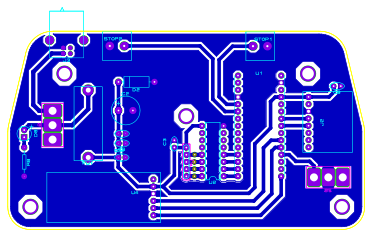
\includegraphics[width=\linewidth]{figuras/desPlataforma/BDT_TCC_rev4}
	\label{fig:BDT_TCC_rev4}
	\fonte{Autor.}
\end{figure}




\subsection{\textit{Layout} da PCI}
O \textit{layout} foi desenvolvido utilizando o espaço reservado na base inferior e nos locais de fixação, respeitando as limitações dos protocolos de comunicação e recomendações de desenvolvimento para os componentes. São cinco pontos de fixação, dos quais quatro localizam-se em cada canto, e o quinto foi instalado no centro, onde planejou-se deixar o conector do motor de passo. O conector USB do tipo B e botões de controle foram posicionados próximos dos cantos da placa. Esses posicionamentos garantem que a placa não irá fletir quando o usuário estiver montando-a ou realizando um acionamento. 

Além desse fator, os componentes foram organizados para serem agrupados em 4 zonas: alimentação, dados, controle e comunicação \textit{Bluetooth} (Figura \ref{fig:zonasPcb}). Buscou-se manter a zona de dados o mais distante possível do sistema \textit{Bluetooth}, e o mais próximo possível do Arduíno, para reduzir a impedância das linhas SDA e SCL do protocolo I2C dos sensores.

\begin{figure}[!htb]
	\centering
	\caption{Regiões da PCB}
	\includegraphics[width=0.7\linewidth]{figuras/desPlataforma/zonasPCB}
	\label{fig:zonasPcb}
	\fonte{Autores.}
\end{figure}  

Foi criado um plano de terra apenas na parte inferior da placa, onde os componentes são soldados. Assim, a placa pode ser fabricada em modos mais simples e artesanais. Por isso, também, manteve-se uma distância de $ 0,75 cm $ entre trilhas, e dos componentes com o plano de terra, visto que distâncias menores podem incorrer em curtos durante o processo de fabricação. A Figura \ref{fig:pcbBot} mostra o projeto da PCI.

\begin{figure}[!htb]
	\centering
	\caption{Projeto da placa de circuito impresso}
	\includegraphics[width=0.7\linewidth]{figuras/desPlataforma/pcbBot}
	\label{fig:pcbBot}
	\fonte{Autor.}
\end{figure}


\subsection{Fabricação do Circuito}
A placa foi fabricada com CNC e os componentes, todos PTH (\textit{Pin Through Hole}), foram soldados com ferro de solda e estanho. Após esses processos, foi aplicado um verniz isolante de PCI -- Isotec \textregistered ~-- da Implastec, para protegê-la contra umidade, visto que a plataforma será usada em ambientes noturnos, ficando exposta ao orvalho e sereno.

\section{Software Embarcado}

As instruções do ATMEGA328p foram desenvolvidas em C++ na IDE do Arduino, e são o \textit{software} que irá embarcar o microcontrolador\footnote{O código está disponível no Github neste \textit{link}: LINK AQUI}. Foram utilizadas bibliotecas adquiridas no GitHub\footnote{As licenças para uso dessas bibliotecas foram respeitadas em conjunto com o licenciamento do projeto} para os sensores, comunicação e controle do motor. Elas foram adaptadas e organizadas para simplificar o código, tornando-o mais eficiente. 

A eletrônica tem como principais funções realizar o controle do motor, ler e processar os dados dos sensores inerciais, enviando os dados dos ângulos calculados para o aplicativo\footnote{As informações sobre o processamento e protocolo de comunicação implementados estão na seção \ref{sec:btandroid}}. Além disso, deve processar o controle dos botões pelo usuário, tanto os botões físicos, como os botões virtuais do aplicativo, cuja alternância de estado é processada na comunicação Bluetooth. 

O processamento dos dados dos sensores inerciais foi implementado com os algoritmos descritos na seção \ref{sec:calcPitchRoll}, para o cálculo de \textit{Pitch} e \textit{Roll}; e seção \ref{sec:azimutal} para algoritmo de cálculo do ângulo azimutal com o magnetômetro. As informações de calibração do magnetômetro foram armazenadas na EEPROM do ATMEGA328P, onde foram utlizados 12 dos 1024 bytes disponíveis \cite{man:atmegadatasheet}.

O módulo de sensores usa comunicação I2C, enquanto o módulo Bluetooth utiliza comunicação UART. O código que implementa a comunicação com esses módulos está descrito nas bibliotecas, respectivamente. O algoritmo dessas bibliotecas está em consonância com o descrito nas seções \ref{sec:uart} e \ref{sec:i2c}.


\chapter{Desenvolvimento do Aplicativo}

\section{Necessidades dos Usuários}

Descrever as necessidades e requisitos mínimos da aplicação. Casos de uso.

\section{Prototipação das Telas}

Escrever sobre a prototipação no Adobe XD

\section{Implementação do Aplicativo Android}

\subsection{Requisitos de Sistema}

Requisitos de Sistema, versão mínima do Android, permissões exigidas pelo usuário, etc.

\subsection{Arquitetura do Funcionamento}

\subsubsection{\textit{Activity}}
\subsubsection{\textit{Room Database}}

Base de dados criadas e valores armazenados


\subsubsection{\textit{Fragments}}

\paragraph{\textit{View Model}}

Databinding

\subsubsection{Protocolo de Comunicação \textit{Bluetooth}}

Diagrama de comunicação, comandos, timeout, checagem de dados, buffer e delay, taxa de atualização e limitações.

\chapter{Resultados Obtidos}

Para validar o sistema é preciso testar os requisitos: mecânicos, de custo, e de desempenho do aplicativo atuando em conjunto com a eletrônica. Então, foram realizados uma sequência de testes em campo. Além disso, a plataforma fora enviada para um astrofotógrafo e Engenheiro, convidado, que conduziu testes usando seu equipamento.\footnote{Relatório do Astrofotógrafo Ricardo Batista pode ser acessado neste link: LINK AQUI}

\section{Requisitos mecânicos}

Os objetivos mecânicos da plataforma foram alcançados com ressalvas. A plataforma montada totalizou 716g sem o \textit{Ball Head} da câmera, estando dentro da faixa de peso comparando com dispositivos similares no mercado. Ademais, a impressão 3D não se comportou como o esperado; somado a isso, existe um erro de inconsistência e vibração motivado por falha de fabricação na barra de elevação curva que deve ser analisado.


\subsection{Impressão 3D}
A engrenagem menor é o elo mais fraco no sistema de transmissão, que se deve pelo seu tamanho mais reduzido. A primeira versão da impressão 3D acabou sofrendo um rachamento por não suportar o torque do motor. Na Figura \ref{fig:engrenagem} é possível verificar que o rasgo se forma perpendicularmente com a tangente da engrenagem, evidenciando esse motivo de ruptura.

\begin{figure}[htb]
	\centering
	\caption{Engrenagem com rachamento em evidência}
	\includegraphics[width=0.25\linewidth]{figuras/resultados/engrenagem}
	\label{fig:engrenagem}
	\fonte{Autor.}
\end{figure}

Além disso, quando a engrenagem apresentou a rachadura, o peso do sistema totalizava mais de 2,5kg com o \textit{Ball-Head }Maxxi Grua somado à câmera CANNON 6D MARK II com uma lente 70-200mm. Contudo, este acontecimento não invalida o projeto pois ocorreu com um peso de rastreamento superior a meta proposta, e, por isso, recomenda-se cautela em situações onde o equipamento se aproxima ou ultrapassa a marca de 2,5kg de peso total.
 

\subsection{Eixo Curvado}
Além do problema com a engrenagem, o movimento de elevação da barra roscada se mostrou inconstante em certos pontos. Essa variação reflete a não idealidade da curvatura dessa barra. A Figura \ref{fig:validaçãoBarraRoscada} torna claro a discrepância entre como deveria ser, e como ficou. Esse erro de fabricação gerou inconsistência em certos pontos no funcionamento da plataforma, e eles serão demonstrados na próxima seção.

\begin{figure}[htb]
	\centering
	\caption{Erro de fabricação demarcado em vermelho, onde a barra apresenta uma curvatura que varia em relação ao desenho técnico}
	\includegraphics[width=0.8\linewidth]{figuras/resultados/validaçãoBarraRoscada}
	\label{fig:validaçãoBarraRoscada}
	\fonte{Autor.}
\end{figure}


\subsection{Análise de Consistência}
\label{sec:vibracao}

A velocidade e vibração da plataforma foram analisados por meio de um sensor acelerômetro instalado na base superior, como demonstra a Figura \ref{fig:sensorInstaladoPlataforma}. Com esse teste, foi possível comparar diferentes cenários de uso de elementos amortecedores no sistema e o seu impacto na consistência e vibração. Os dados foram obtidos em uma taxa de 100Hz, utilizando um Arduíno e comunicação Serial com um notebook que armazenava os dados \footnote{O sistema de captação de dados com o sensor está documentado neste repositório do Github: Link AQUI}. 

\begin{figure}[htb]
	\centering
	\caption{Sensor instalado na base superior}
	\includegraphics[width=0.35\linewidth]{figuras/resultados/sensorInstaladoPlataforma}
	\label{fig:sensorInstaladoPlataforma}
	\fonte{Autor.}
\end{figure}

Então, os dados obtidos no primeiro teste -- que constam na Figura \ref{fig:antes} --, demonstram que existia uma inconstância na velocidade angular do sistema, além de um excesso de vibração. Além disso, com os dados da Figura \ref{fig:depois}, confirmou-se que existe a necessidade de elementos para dissipar a vibração. Ressalta-se ainda que existem pontos de intensificação da vibração, e, pelo período temporal onde acontece, é possível inferir que são decorrentes do erro de fabricação do eixo curvado. 

\begin{figure}[!htb]
	\centering
	\caption{Primeiro teste do sistema}
	\includegraphics[width=0.9\linewidth]{figuras/resultados/antes}
	\label{fig:antes}
	\fonte{Autor.}
\end{figure}

\begin{figure}[!htb]
	\centering
	\caption{Teste do sistema com elementos amortecedores}
	\includegraphics[width=0.9\linewidth]{figuras/resultados/depois}
	\label{fig:depois}
	\fonte{Autor.}
\end{figure}

\section{Custo total do sistema}
O custo dos materiais e processos de fabricação estão descritos na tabela \ref{table:custo}\footnote{Alguns valores são aproximados pois foram doados pela Universidade}, com a qual pode se constar um total de 305 reais envolvendo materiais e fabricação de componentes. Comparando ao valor do NyxTech -- que possui uma construção e materiais similares, com um preço de US\$ 110 -- o EasyTracker conseguiu vencer a meta de custo.  

\begin{table}[!htb]
	\centering
	\caption{Descrição aproximada dos Custos do Sistema}
	\begin{tabular}{c|c}
	Item	&	Custo	\\\hline\hline
	MDF	15mm	&	R\$ 25,00		\\\hline
	Corte a Laser			&	R\$ 100,00		\\\hline
	PCB			&	R\$ 50,00		\\\hline
	Componentes Eletrônicos			&	R\$ 95,00		\\\hline
	Outros Materiais		&	R\$ 35,00		\\\hline\hline
	Total			&	R\$ 305,00		\\
	\end{tabular}
	\label{table:custo}
	\fonte{Autor.}
\end{table}


\section{Análise de desempenho do aplicativo}
O \textit{software} pode ser avaliado com relação ao uso e implementação das heurísticas de desenvolvimento, com relação ao desempenho em \textit{hardware} -- consumo de processamento e memória --, e ainda pode ser avaliado com \textit{feedbacks} dos usuários. 

\subsection{Interface Gráfica}
Quando à interface e recursos, é possível avaliar de forma qualitativa como as 10 Heurísticas de Nielsen foram utilizadas. Os status cruciais para funcionamento são todos visíveis: o \textit{status} \textit{bluetooth} do sistema é visível por meio do estado do botão de conexão na tela de visualização do perfil. Nas telas de alinhamento, se o sistema está alinhado, os ícones ficam esverdeados, caso contrário ficam avermelhados.

Além disso, as cores e os elementos de ícones são similares com o que os usuários estão acostumados, como os ícones nas telas de perfis de localização que fazem sentido para o contexto e são minimalistas. Além disso, as telas de alinhamento se assemelha a uma bolha de nível onde o acelerômetro é empregado. Na tela de alinhamento com o polo magnético, o sistema emula uma bússola. 

Nessas mesmas telas de alinhamento, os usuários podem controlar livremente o fluxo das telas de alinhamento. Dessa forma conseguem conferir alguma informação que possam ter ignorado, assim como podem navegar para telas de suporte. Não obstante, a consistência desses padrões nas telas de alinhamento também foi consolidado nas telas de perfis. As ações de criar, editar, e visualizar um perfil usam por base a mesma tela, facilitando para o usuário entender como utilizar o aplicativo. 

Além disso, a prevenção de erros é feita de forma ativa relembrando o usuário de, por exemplo, calibrar a bússola ao entrar na tela de alinhamento azimutal, ou também com um \textit{popup} para atualizar os dados de declinação magnética em localizações que foram armazenadas e não foram atualizadas por mais e 2 meses. A prevenção também ocorre nas entradas de dados:  onde o usuário precisa inserir valores de latitude e declinação, que devem ser valores decimais (Figura \ref{fig:gpsedit}). No entanto, eles podem ser escritos em graus, minutos e segundos, mas o usuário não vai conseguir inserir dessa forma, pois, o teclado numérico não permite essa formatação.

\begin{figure}[!htb]
	\centering
	\includegraphics[width=0.3\linewidth]{figuras/resultados/gpsedit}
	\caption{Teclado só permite uso de vírgula e ponto, não permitindo aspas e sinal de grau $ (^\circ) $}
	\label{fig:gpsedit}
\end{figure} 

Dessa forma, o desenvolvimento da interface gráfica do aplicativo conseguiu atingir um estágio de desenvolvimento compatível com o estado da arte atual relativo a criação de aplicativos Android ou outros Softwares. As heurísticas foram respeitadas e a implementação é fluída, os itens estão dispostos respeitando uma hierarquia visual que está em conluio com a identidade do projeto e os recursos do Sistema Android. 

\subsection{Desempenho}
O aplicativo foi lançado na loja de aplicativos Android via Google Play Console. O Console de desenvolvedor realiza testes automáticos com alguns dispositivos e avalia o desempenho. Os resultados indicam que o aplicativo pode ter problemas de lentidão em hardwares mais antigos e com menor capacidade de memória e armazenamento; mas, ao mesmo tempo, não detectou nenhum problema em sistemas mais recentes (Figura \ref{fig:relatorioDesempenho}).

\begin{figure}[htb]
	\centering
	\caption{Resultados apresentados no Google Play Console}
	\includegraphics[width=\linewidth]{figuras/resultados/relatorioDesempenho}
	\label{fig:relatorioDesempenho}
	\fonte{Autor.}
\end{figure}

Considerando que o dispositivo com dificuldade no processamento é defasado, é razoável considerar que o aplicativo não trará problema para a maior parcela de dispositivos. 

\section{Comparativo Geral}
Os 3 pontos avaliados anteriormente listam eventuais problemas que afetaram a consistência do sistema e projeto como um todo. No entanto, é necessário verificar ainda se, apesar desses entraves, o projeto consegue cumprir com os objetivos gerais: se o método de alinhamento é tão confiável quanto os métodos tradicionais de luneta e laser; assim como se as especificações de erro estão dentro da margem comercial. Dessa maneira, dois erros podem ser avaliados: o erro inerente ao sistema mecânico, nomeado de erro periódico; e o erro relativo ao processo de alinhamento.


\subsection{Erro Periódico}

O erro periódico mensura a oscilação do sistema de transmissão, gerada por variações na montagem e encaixe dos componentes. O período desse erro é definido pelo tempo total levado para que o motor de passo realize 1 rotação. O erro é medido em arco-segundos (arcsec), que é uma unidade que irá avaliar o quanto uma estrela alternou sua posição pelo visor da câmera, em uma fração de graus, independente da lente utilizada. O teste que mensura esse erro é realizado apontando a câmera para qualquer alvo no céu, desalinhando o rastreador propositalmente, e realizando uma fotografia de longa exposição \cite{site:nyxtechFAQPeriodicError}. 

Então, apontou-se a câmera para Júpiter, utilizando a Câmera DSC-HX300, com comprimento focal em $ d = 192~mm $, e assim fora possível extrair a seguinte oscilação do posicionamento da estrela ao longo de 8 fotografias captadas em intervalos de 10s. Empilhando as imagens, têm-se o resultado da Figura \ref{fig:periodicErrorImage}. Usando um software editor de imagens, é possível desenhar sobre esses pontos uma forma de onda. O erro periódico é igual a distância de pico a pico medida em arc segundos. Essa distância é medida inicialmente em pixel, e posteriormente convertida para arcsec com as equações (\ref{eq:arc}) e (\ref{eq:erroperiodic}), sabendo que essa câmera tem um tamanho de pixel ($ px_s $) igual a  $ 1,19~um $ e sendo $ d_{AB} $ a distância em pixel pico a pico da onda. Esse procedimento foi realizado também com outros equipamentos, e com diferentes alvos, e a média de erro periódico calculado foi igual  $ 63~arcsec  $. Os resultados documentados podem ser conferidos no apêndice \ref{apendice:periodic}.


\begin{equation}
	ang_{Res}~(arcsec/px) = \dfrac{px_s~ (\mu m) * 206,3}{d~ (mm)}
	\label{eq:arc}
\end{equation}

\begin{equation}
	Erro_{periodico}~(arcsec) = d_{AB}~(px) \times ang_{Res} ~(arcsec/px)
	\label{eq:erroperiodic}
\end{equation}

\begin{figure}[htb]
	\centering
	\caption{Pontos obtidos com as 8 imagens sobrepostas, que foram captadas com intervalos de 10s}
	\includegraphics[width=.8\linewidth]{figuras/resultados/periodicErrorImage}
	\label{fig:periodicErrorImage}
	\fonte{Autor.}
\end{figure}


\subsection{Erro de Alinhamento}

Um alinhamento bem feito está diretamente relacionado ao tempo de exposição máximo de uma foto registrada com a câmera montada no EasyTracker. Segundo o convidado Ricardo Batista, em seu relatório, o iOptron SkyGuider Pró consegue proporcionar até 4 \textit{stops} extras de exposição, com um alinhamento pela luneta. Isso significa dizer que o tempo total de exposição que é possível atingir com rastreamento é de $ t_{max} = t_{atual} \times 2^{stop = 4} $; onde o $ t_{atual} $ é o tempo utilizado para fotografias sem rastreamento. 


Para determinar quantos "\textit{stops}" é possível atingir, é necessário avaliar o erro de rastreamento da plataforma ao longo de um período de tempo. Com base nesse erro, determina-se o tempo máximo de exposição para que a estrela não passe de um limite de tolerância especificado pela Regra NPF (seção \ref{sec:regraNPF}). Essa tolerância indica quantos pixeis uma estrela pode mover-se na captura da imagem, sem que isso seja um rastro indesejável. Assim, com o erro determinado, compara-se o tempo pela regra NPF e o tempo de rastreamento máximo estimado pelos valores empíricos; calculando quantos stops extras são possíveis de se obter com o alinhamento da plataforma.

Então, em diferentes condições e câmeras, foram realizadas diversas capturas, anotando o tempo de intervalo entre elas. Todas fotografias foram realizadas com o rastreador ligado e alinhado. Com elas, foi possível determinar quantos pixeis a estrela deslocou no período de tempo observado, obtendo, com isso, a velocidade angular de erro. Com a equação (\ref{eq:arc}) utilizada na seção anterior, determina-se a resolução angular da câmera, e pode-se então determinar quantos arcsec/s de erro acumula-se durante o rastreamento do EasyTracker.

Com a regra NPF, então, determina-se o tempo de exposição correto para que não haja rastro, $ tmax_{NPF} $. Sabendo a resolução angular da câmera e a velocidade angular da terra em arcsec/s calculado na equação (\ref{eq:arcsecTerra}), determina-se a tolerância do rastro de pixeis, $ NPF_{tol.} $,  com a regra NPF com a equação (\ref{eq:tolerancia}). 

\begin{equation}
	V_{terra} = \dfrac{360 \cdot 3600}{23\cdot3600+55\cdot60 + 4} = 15,04~arcsec/s
	\label{eq:arcsecTerra}
\end{equation}

\begin{equation}
	NPF_{tol.} = \dfrac{tmax_{NPF} ~\left[s\right]\cdot V_{terra}}{ang_{Res}~\left[arcsec/px\right]}~\left[px\right]
	\label{eq:tolerancia}
\end{equation}

Dessa maneira, calcula-se o tempo máximo, $ t_{max} $, de rastreamento com a equação (\ref{eq:tmax}) sabendo: o erro de rastreamento do sistema, $ V_{erro} $; a tolerância de pixeis $ NPF_{tol.} $; e a resolução angular da câmera, $ ang_{Res}~\left[arcsec/px\right] $. Esse resultado, quando comparado ao tempo dado pela regra NPF, determina quantos stops de exposição foi possível obter com o EasyTracker. 

\begin{equation}
	t_{max} = \dfrac{NPF_{tol.}\cdot ang_{Res} }{V_{erro}} \left[s\right]
	\label{eq:tmax}
\end{equation}

Nos testes mais recentes, possuindo prática com o equipamento, fora possível obter até $ 4,46 $ stops de exposição. O apêndice \ref{apendice:alignment} contém uma tabela registrando as medidas obtidas com cada captura realizada em testes. 

Os testes conduzidos pelo convidado também levaram à marca de 4 stops. Também foi possível verificar que o método do aplicativo é muito mais ágil quando comparado aos tradicionais, podendo ser realizado em até quatro minutos. Isso é quatro vezes mais rápido comparando com o tempo necessário para alinhamento realizado usando a luneta do iOptron SkyGuider Pro e executado por um profissional experiente. 

\chapter{Considerações Finais}

\section{Projeto \textit{Open-Source}}


	
	
% % % % % % % % % % % % % % % % % % % % % % % % % % % % % % % % % % % % % % 
% % % % % % % % % % % % FIM DAS PAGINAS TEXTUAIS % % % % % % % % % % % % % % 
% % % % % % % % % % % % % % % % % % % % % % % % % % % % % % % % % % % % % % 



% % % % % % % % % % % % % % % % % % % % % % % % % % % % % % % % % % % % % % 	
% % % % % % % % % % % % % BIBLIOGRAFIA  % % % % % % % % % % % % % % % % % % 
% % % % % % % % % % % % % % % % % % % % % % % % % % % % % % % % % % % % % % 	

\bibliography{referencias}  %%%%% BIBLIOGRAFIA -> INCLUIR NAS CHAVES O NOME DO ARQUIVO *.BIB

%\bibliografia{referencias}	
	
	
	
% % % % % % % % % % % % % % % % % % % % % % % % % % % % % % % % % % % % % 	
% % % % % % % % % % % % % APENDICES % % % % % % % % % % % % % % % % % % %
% % % % % % % % % % % % % % % % % % % % % % % % % % % % % % % % % % % % % 	

\apendice %%%% TEXTOS A PARIR DESTE PONTO SERAO CONSIDERADOS APENDICES

\chapter{Desenho Técnico das Peças}

\section{Base}

\includegraphics[width=\linewidth]{E:/Git/Easy-Tracker-System/CAD/Fabricação/BDT_I_P_11_v01_desenho}

\section{Parte Móvel}

\section{Barra curvada}

\includegraphics[width=\linewidth]{E:/Git/Easy-Tracker-System/CAD/Fabricação/BDT_G_F_05_v01_desenho}

\chapter{Diagrama de Montagem}

%\chapter{Código excutado pelo Arduino Nano}


%\arduinominted{configuration.h}

%\arduinominted{HMC5883L_bdt.cpp}
%\arduinominted{HMC5883L_bdt.h}
%\arduinominted{MPU6050_bdt.cpp}
%\arduinominted{MPU6050_bdt.h}
%\arduinominted{stp.cpp}
%\arduinominted{stp.h}

%\arduinominted{bluetooth.ino}
%\arduinominted{debug.ino}
%\arduinominted{sensorData.ino}
%\arduinominted{i2c.ino}
%\arduinominted{main.ino}

%\chapter{Código do Aplicativo (Sem as Telas)}

%\section{Rotina da Atividade Principal}
%\kotlinminted{MainActivity.kt}
%\kotlinminted{Util.kt}

%\section{Layout da Atividade Principal}
%\xmlminted{activity_main.xml}

%\section{Classe Bluetooth}
%\kotlinminted{BluetoothService.kt}




% % % % % % % % % % % % % % % % % % % % % % % % % % % % % % % % % % % % % % 	
% % % % % % % % % % % % % % % ANEXOS  % % % % % % % % % % % % % % % % % % % 
% % % % % % % % % % % % % % % % % % % % % % % % % % % % % % % % % % % % % % 	

%\anexo    %%%% TEXTOS A PARIR DESTE PONTO SERAO CONSIDERADOS ANEXOS
        
%\chapter{Algo interessante que alguém fez}
      
         
\end{document}
